\section{Results of the \MET\ Templates Analysis}
\label{sec:templates}

In this section, we use the \MET\ templates technique to derive predictions for the Z background in the Z mass regions for the 
two signal regions used for the OSSF dilepton analysis. The background estimation methodology used in the \MET\ templates analysis
is described in AN-2012/254; this AN presents only details which differ from that reference. 
We then use the predicted Z background to derive an estimate of the low-mass $\gamma^*$/Z contribution,
using an extrapolation technique commonly referred to as the ``$R_{out/in}$'' technique~\cite{ref:routin}.

\subsection{Background Estimation Methodology}
\label{sec:templates_bkg}

The strategy is to select Z$\to\ell\ell$ candidates ($81<m_{\ell\ell}<101$ GeV) with jet requirements corresponding to the
low-\MET\ and high-\MET\ signal regions, and compare the observed \MET\ distribution to the sum of the predictions from the 
\zjets\ background (from the \MET\ templates method based on the \gjets\ data control sample), the flavor-symmetric (FS) 
background predicted from e$\mu$ data events, and MC contributions from WZ/ZZ (for which the contribution to the FS background 
estimate is negligible), as well as the rare SM processes with 
Z bosons ($t\bar{t}\rm{Z}$ and ZZZ, ZZW, ZWW). The reader is referred to AN-2012/254 for details of the methods.

In order to adapt the \MET\ templates method to predict the Z background in these regions, we make minor modifications
to the procedure used in AN-2012/254. Specifically, we re-calculate
the flavor-symmetric (FS) scaling factor $K$ and change the binning used for the \MET\ templates.
The FS background is estimated using e$\mu$ events in data.
To improve the precision of this background estimate, the dilepton mass requirement is not applied, and we apply a scaling
factor $K$, which is the efficiency for e$\mu$ events to fall in the Z mass window,  extracted from MC.
The systematic uncertainty on $K$ is assessed by comparing this quantity in data vs. MC.
The values of $K$ for various \MET\ intervals for the high-\MET\ region (using \pt\ $>$ (20,10) GeV leptons and at least 2 jets) 
are shown in Fig.~\ref{fig:K_incl_highmet}. 
Based on this plot we choose $K=0.13\pm0.02$ for \MET\ signal regions up to 200 GeV; for \MET\ 200-300 GeV and \MET\ $>$ 300 GeV
we inflate the uncertainty to $K=0.13\pm0.04$ and $K=0.13\pm0.05$, respectively, due to the limited statistical precision.
The values of $K$ for the low-\MET\ region (using \pt\ $>$ (20,20) GeV leptons and at least 3 jets) are shown in 
Fig.~\ref{fig:K_incl_lowmet}. 
Based on this plot we choose $K=0.14\pm0.02$ for \MET\ signal regions up to 200 GeV; for \MET\ 200-300 GeV and \MET\ $>$ 300 GeV
we inflate the uncertainty to $K=0.14\pm0.03$ and $K=0.14\pm0.07$, respectively. In addition, we change the 
jet \pt\ threshold for the \MET\ templates jet multiplicity binning from 30 to 40 GeV, and change the $H_T$ bins to
(0,80,100,150,200,250,300,5000) GeV.

\begin{figure}[!ht]
\begin{center}
\begin{tabular}{cc}
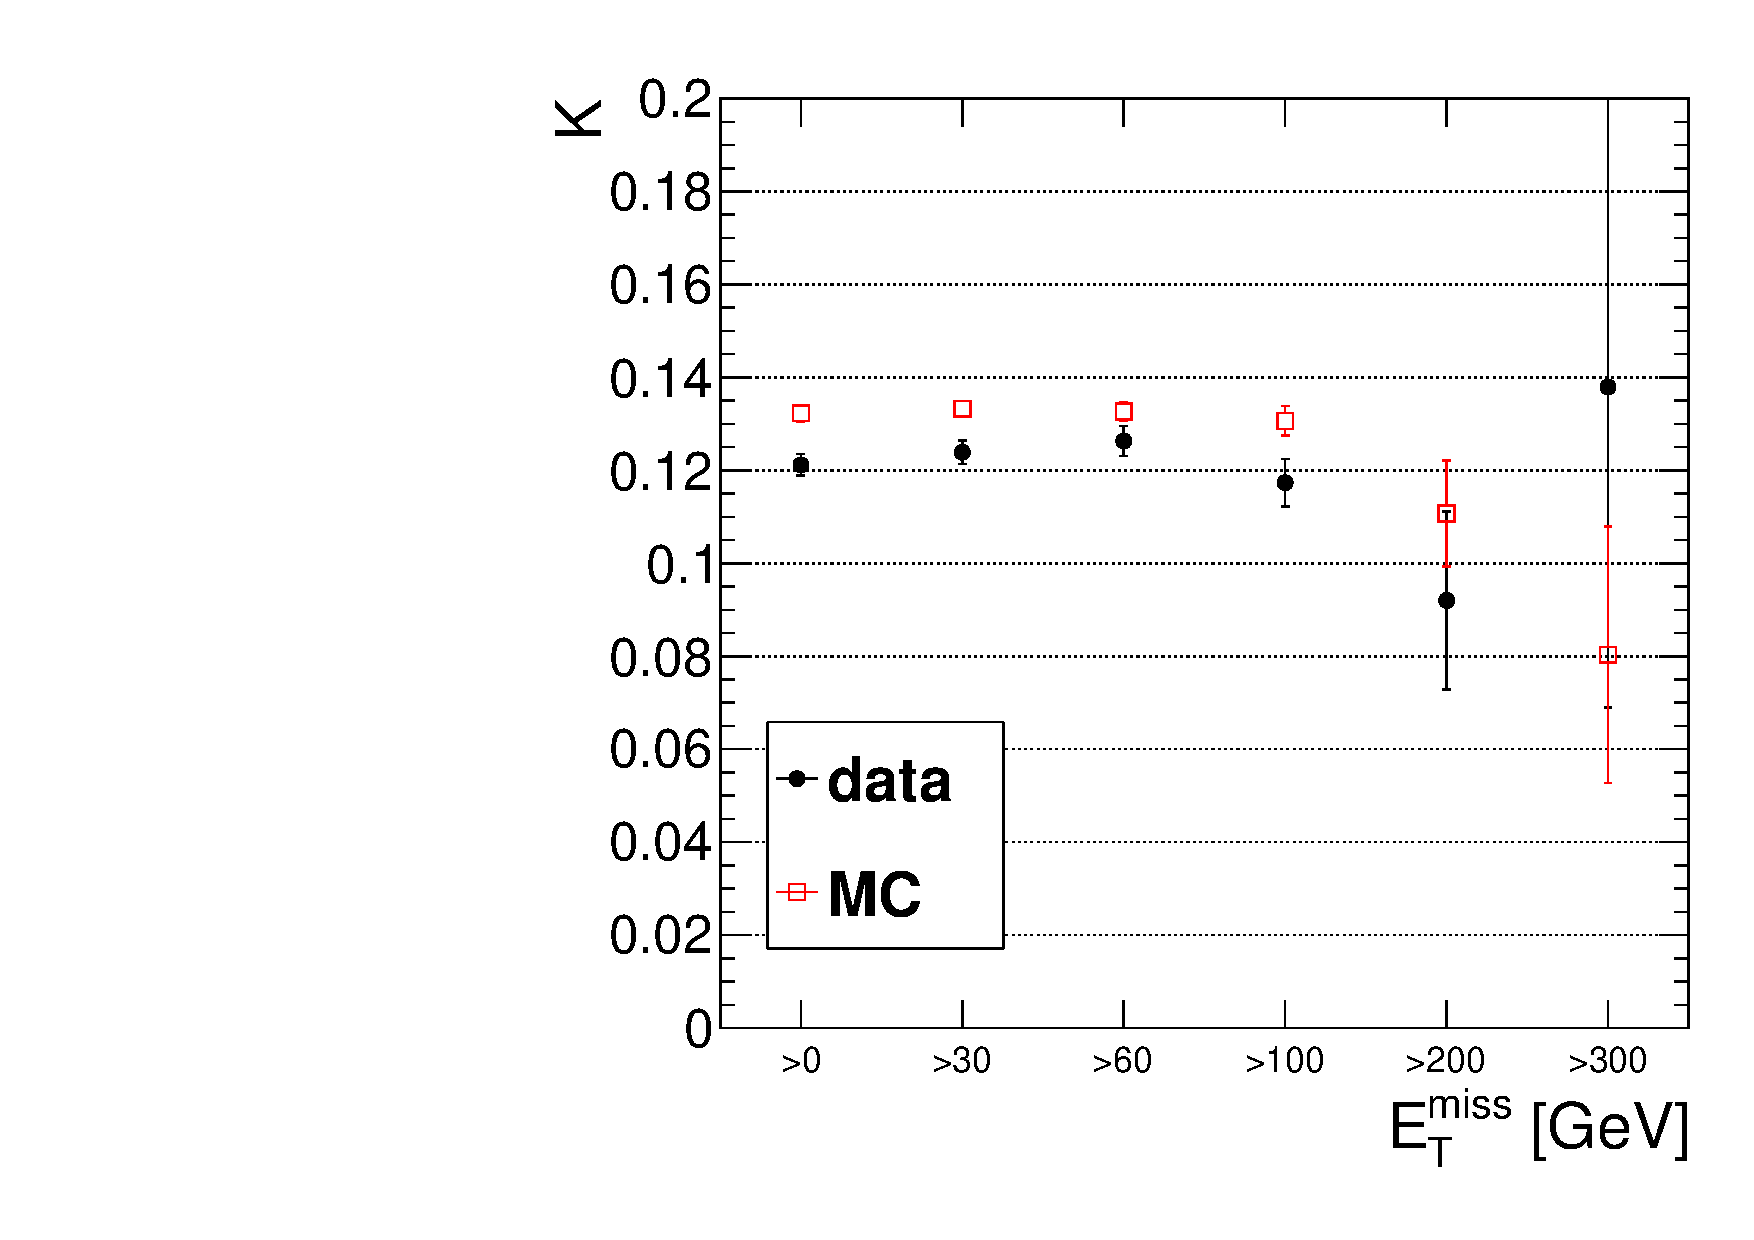
\includegraphics[width=0.4\textwidth]{plots/extractK_inclusive_pt2010_92fb.pdf} &
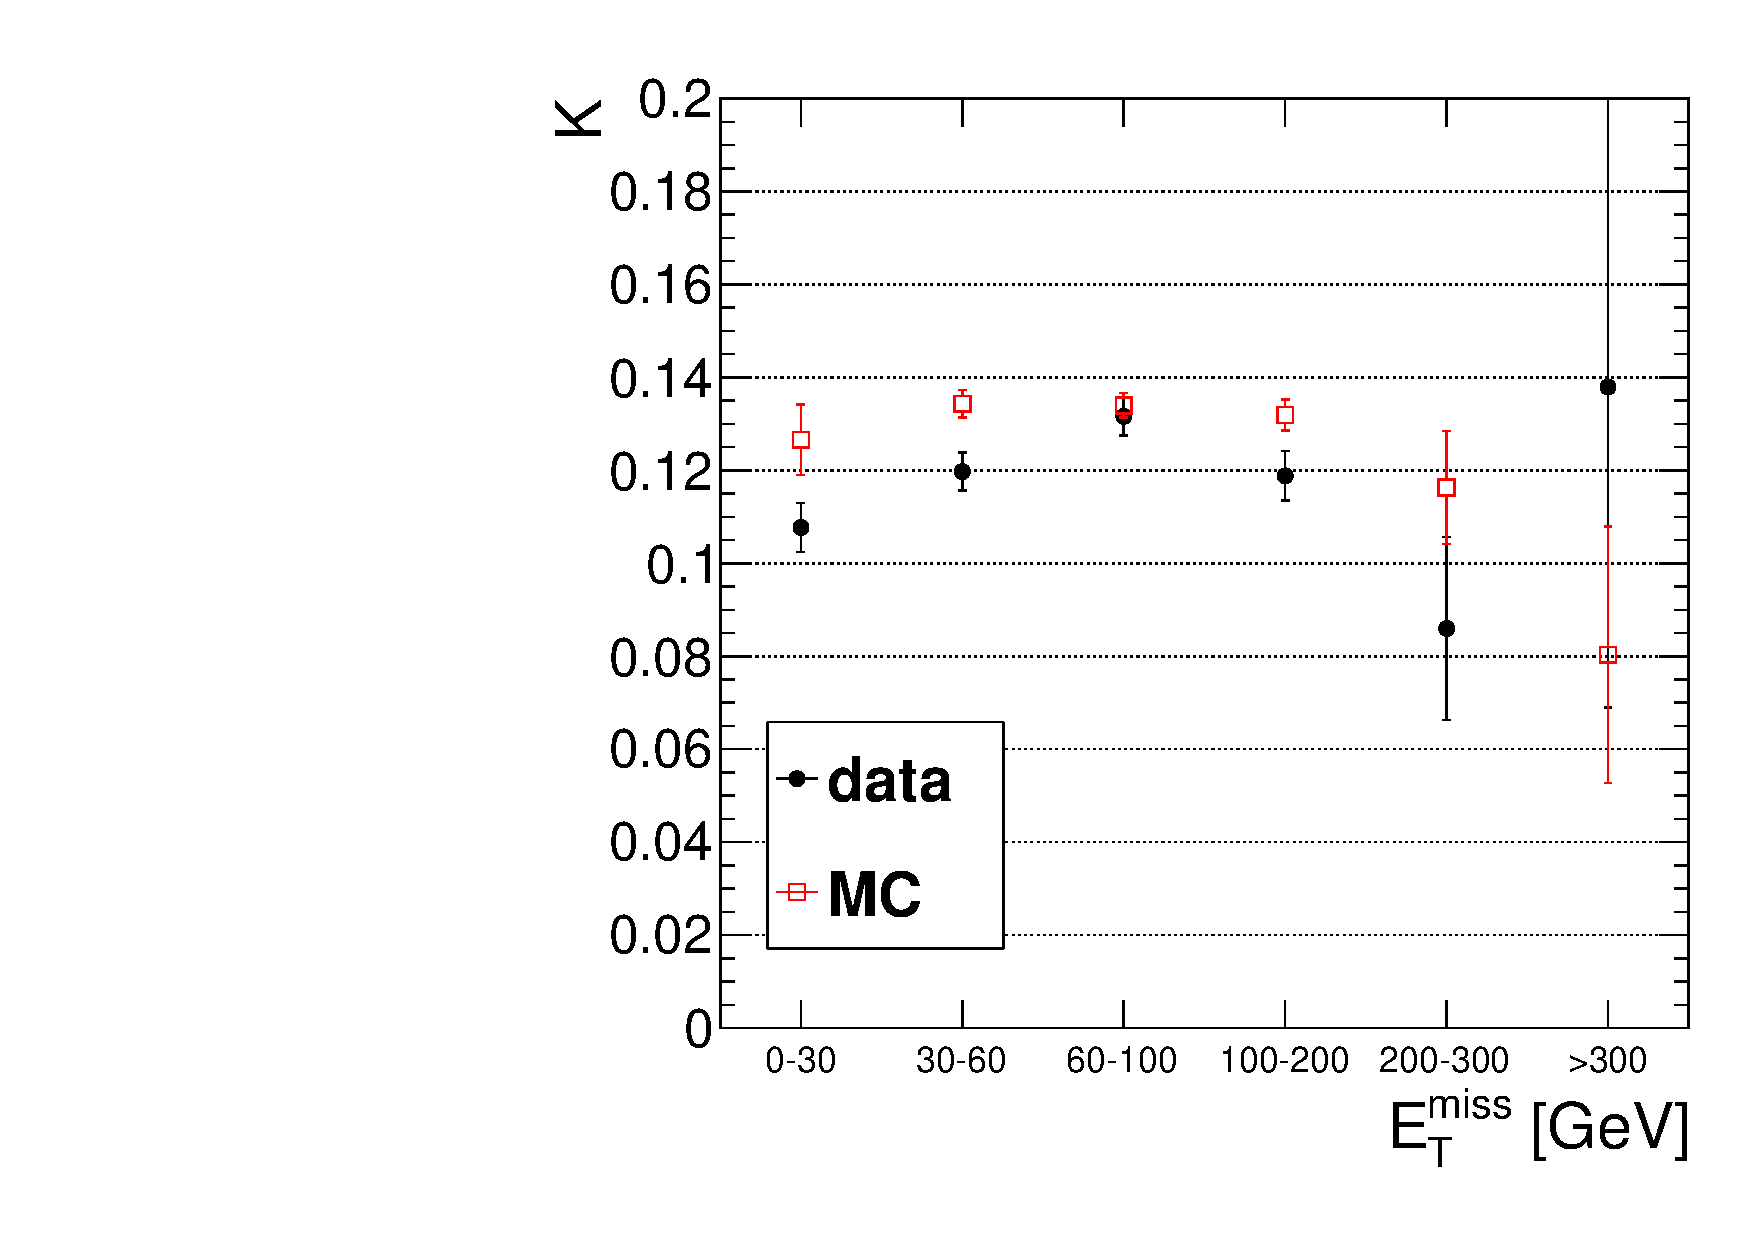
\includegraphics[width=0.4\textwidth]{plots/extractK_exclusive_pt2010_92fb.pdf} \\
\end{tabular}
\caption{\label{fig:K_incl_highmet}
The efficiency for e$\mu$ events to satisfy the dilepton mass requirement, $K$, in data and simulation for inclusive \MET\ intervals 
(left) and exclusive \MET\ intervals (right) for the dilepton \pt\ $>$ (20,10) GeV selection with at least 2 \pt\ $>$ 40 GeV jets
(used for the high \MET\ signal region). 
}
\end{center}
\end{figure}

\begin{comment}

Using selection : ((((leptype==2)&&(csc==0 && hbhe==1 && hcallaser==1 && ecaltp==1 && trkfail==1 && eebadsc==1 && hbhenew==1))&&(isdata==0 || (run<197556 || run>198913)))&&(njets40>=2))&&(lep1.pt()>20 && lep2.pt()>10)
Using weight    : vtxweight * weight
OF entries (total)  23031
OF entries (Z mass) 2791
K                   0.121184
Warning in <TROOT::Append>: Replacing existing TH1: htot (Potential memory leak).
Warning in <TROOT::Append>: Replacing existing TH1: hZ (Potential memory leak).

--------------------------------------------------------------
pfmet>0   && pfmet<30

data  : 
total : 3835
Z     : 413
K     : 0.11 +/- 0.005

MC    : 
total : 378.922
Z     : 47.9593
K     : 0.13 +/- 0.008
--------------------------------------------------------------


--------------------------------------------------------------
pfmet>30  && pfmet<60

data  : 
total : 7090
Z     : 849
K     : 0.12 +/- 0.004

MC    : 
total : 775.198
Z     : 104.129
K     : 0.13 +/- 0.003
--------------------------------------------------------------


--------------------------------------------------------------
pfmet>60  && pfmet<100

data  : 
total : 7598
Z     : 1000
K     : 0.13 +/- 0.004

MC    : 
total : 886.062
Z     : 118.721
K     : 0.13 +/- 0.003
--------------------------------------------------------------


--------------------------------------------------------------
pfmet>100 && pfmet<200

data  : 
total : 4258
Z     : 506
K     : 0.12 +/- 0.005

MC    : 
total : 538.442
Z     : 71.0424
K     : 0.13 +/- 0.003
--------------------------------------------------------------


--------------------------------------------------------------
pfmet>200 && pfmet<300

data  : 
total : 221
Z     : 19
K     : 0.09 +/- 0.020

MC    : 
total : 29.8247
Z     : 3.46834
K     : 0.12 +/- 0.012
--------------------------------------------------------------


--------------------------------------------------------------
pfmet>300

data  : 
total : 29
Z     : 4
K     : 0.14 +/- 0.069

MC    : 
total : 5.45734
Z     : 0.438259
K     : 0.08 +/- 0.028
--------------------------------------------------------------

root [1] extractK(false,false,false)
Using selection : ((((leptype==2)&&(csc==0 && hbhe==1 && hcallaser==1 && ecaltp==1 && trkfail==1 && eebadsc==1 && hbhenew==1))&&(isdata==0 || (run<197556 || run>198913)))&&(njets40>=2))&&(lep1.pt()>20 && lep2.pt()>10)
Using weight    : vtxweight * weight
OF entries (total)  23031
OF entries (Z mass) 2791
K                   0.121184
Info in <TCanvas::MakeDefCanvas>:  created default TCanvas with name c1

--------------------------------------------------------------
pfmet>0

data  : 
total : 23031
Z     : 2791
K     : 0.12 +/- 0.002

MC    : 
total : 2613.71
Z     : 345.768
K     : 0.13 +/- 0.002
--------------------------------------------------------------


--------------------------------------------------------------
pfmet>30

data  : 
total : 19196
Z     : 2378
K     : 0.12 +/- 0.003

MC    : 
total : 2234.8
Z     : 297.807
K     : 0.13 +/- 0.002
--------------------------------------------------------------


--------------------------------------------------------------
pfmet>60

data  : 
total : 12106
Z     : 1529
K     : 0.13 +/- 0.003

MC    : 
total : 1459.78
Z     : 193.67
K     : 0.13 +/- 0.002
--------------------------------------------------------------


--------------------------------------------------------------
pfmet>100

data  : 
total : 4508
Z     : 529
K     : 0.12 +/- 0.005

MC    : 
total : 573.708
Z     : 74.9489
K     : 0.13 +/- 0.003
--------------------------------------------------------------


--------------------------------------------------------------
pfmet>200

data  : 
total : 250
Z     : 23
K     : 0.09 +/- 0.019

MC    : 
total : 35.2821
Z     : 3.90659
K     : 0.11 +/- 0.011
--------------------------------------------------------------


--------------------------------------------------------------
pfmet>300

data  : 
total : 29
Z     : 4
K     : 0.14 +/- 0.069

MC    : 
total : 5.45734
Z     : 0.438259
K     : 0.08 +/- 0.028
--------------------------------------------------------------

\end{comment}


\begin{figure}[!ht]
\begin{center}
\begin{tabular}{cc}
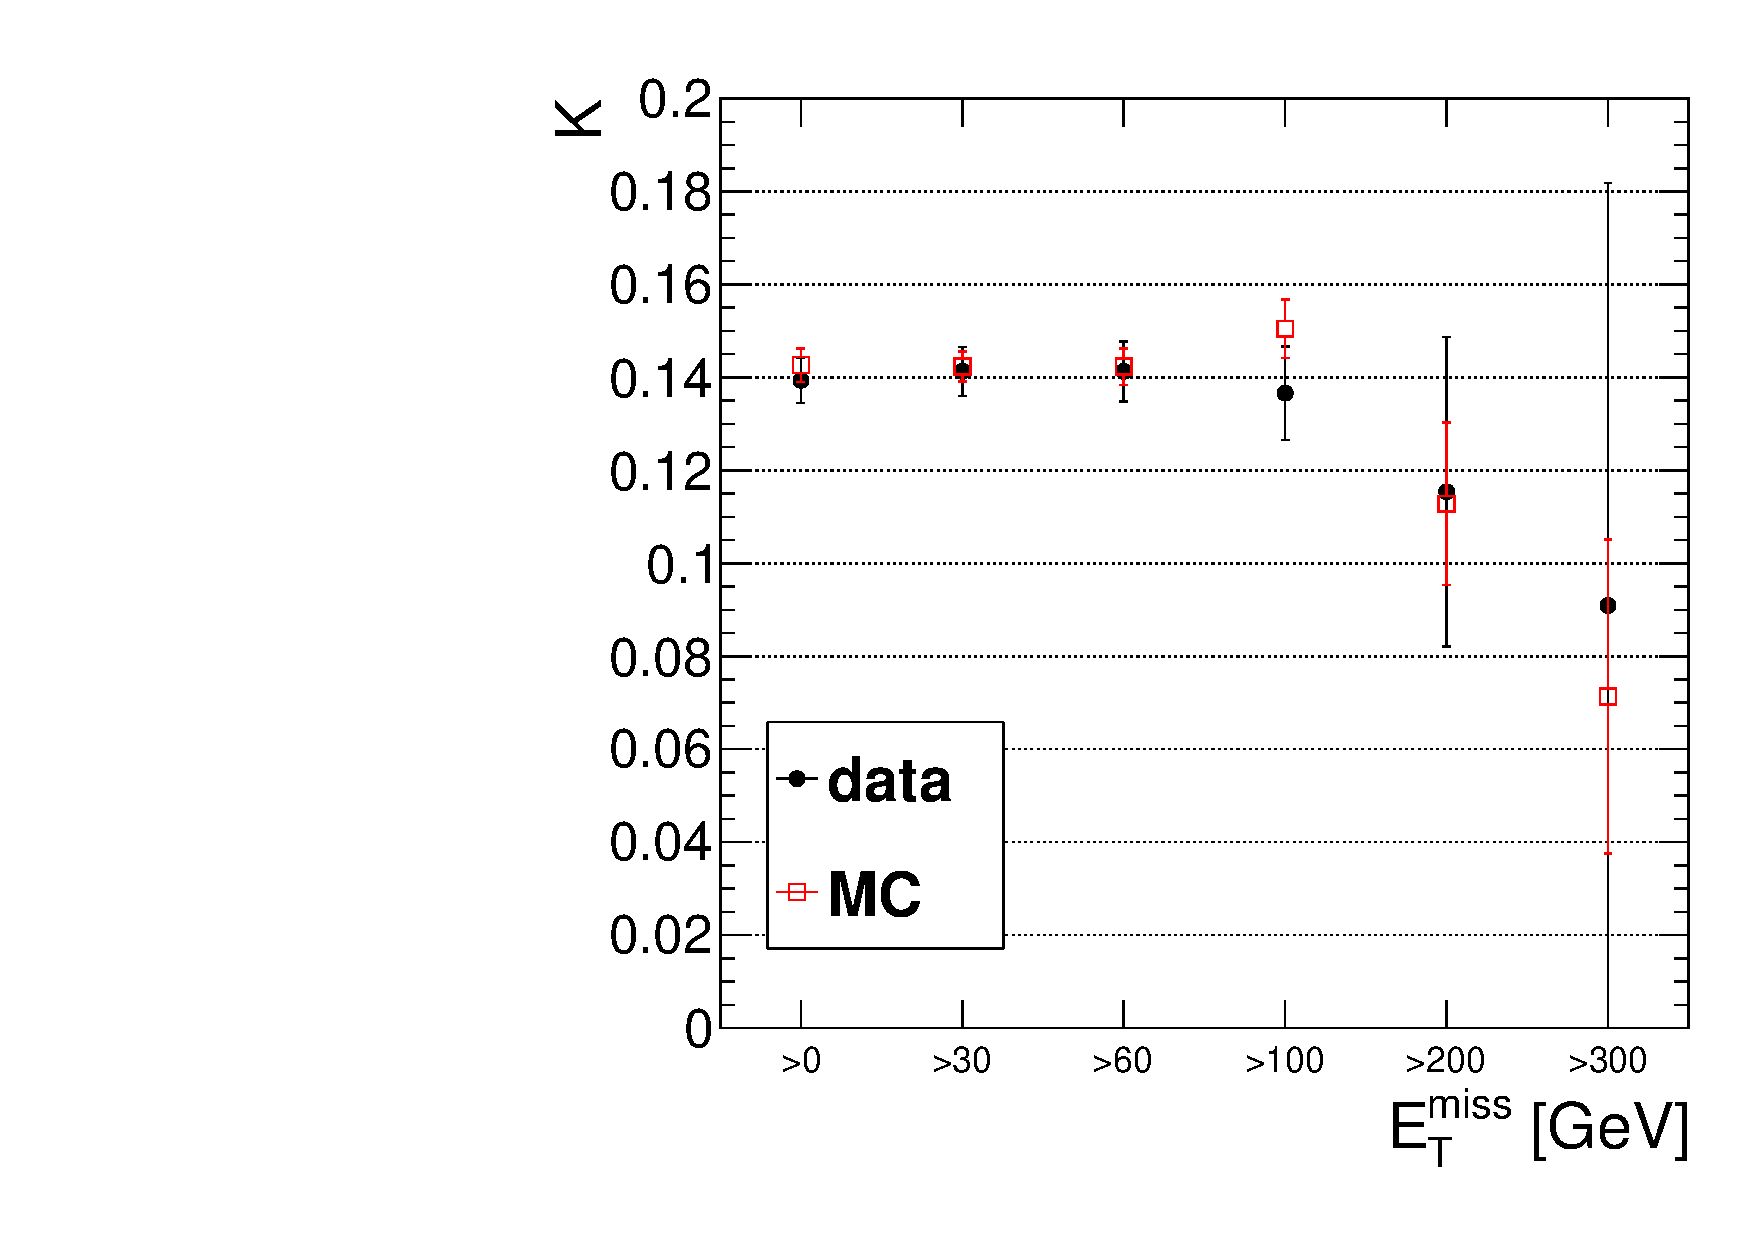
\includegraphics[width=0.4\textwidth]{plots/extractK_inclusive_lowmet.pdf} &
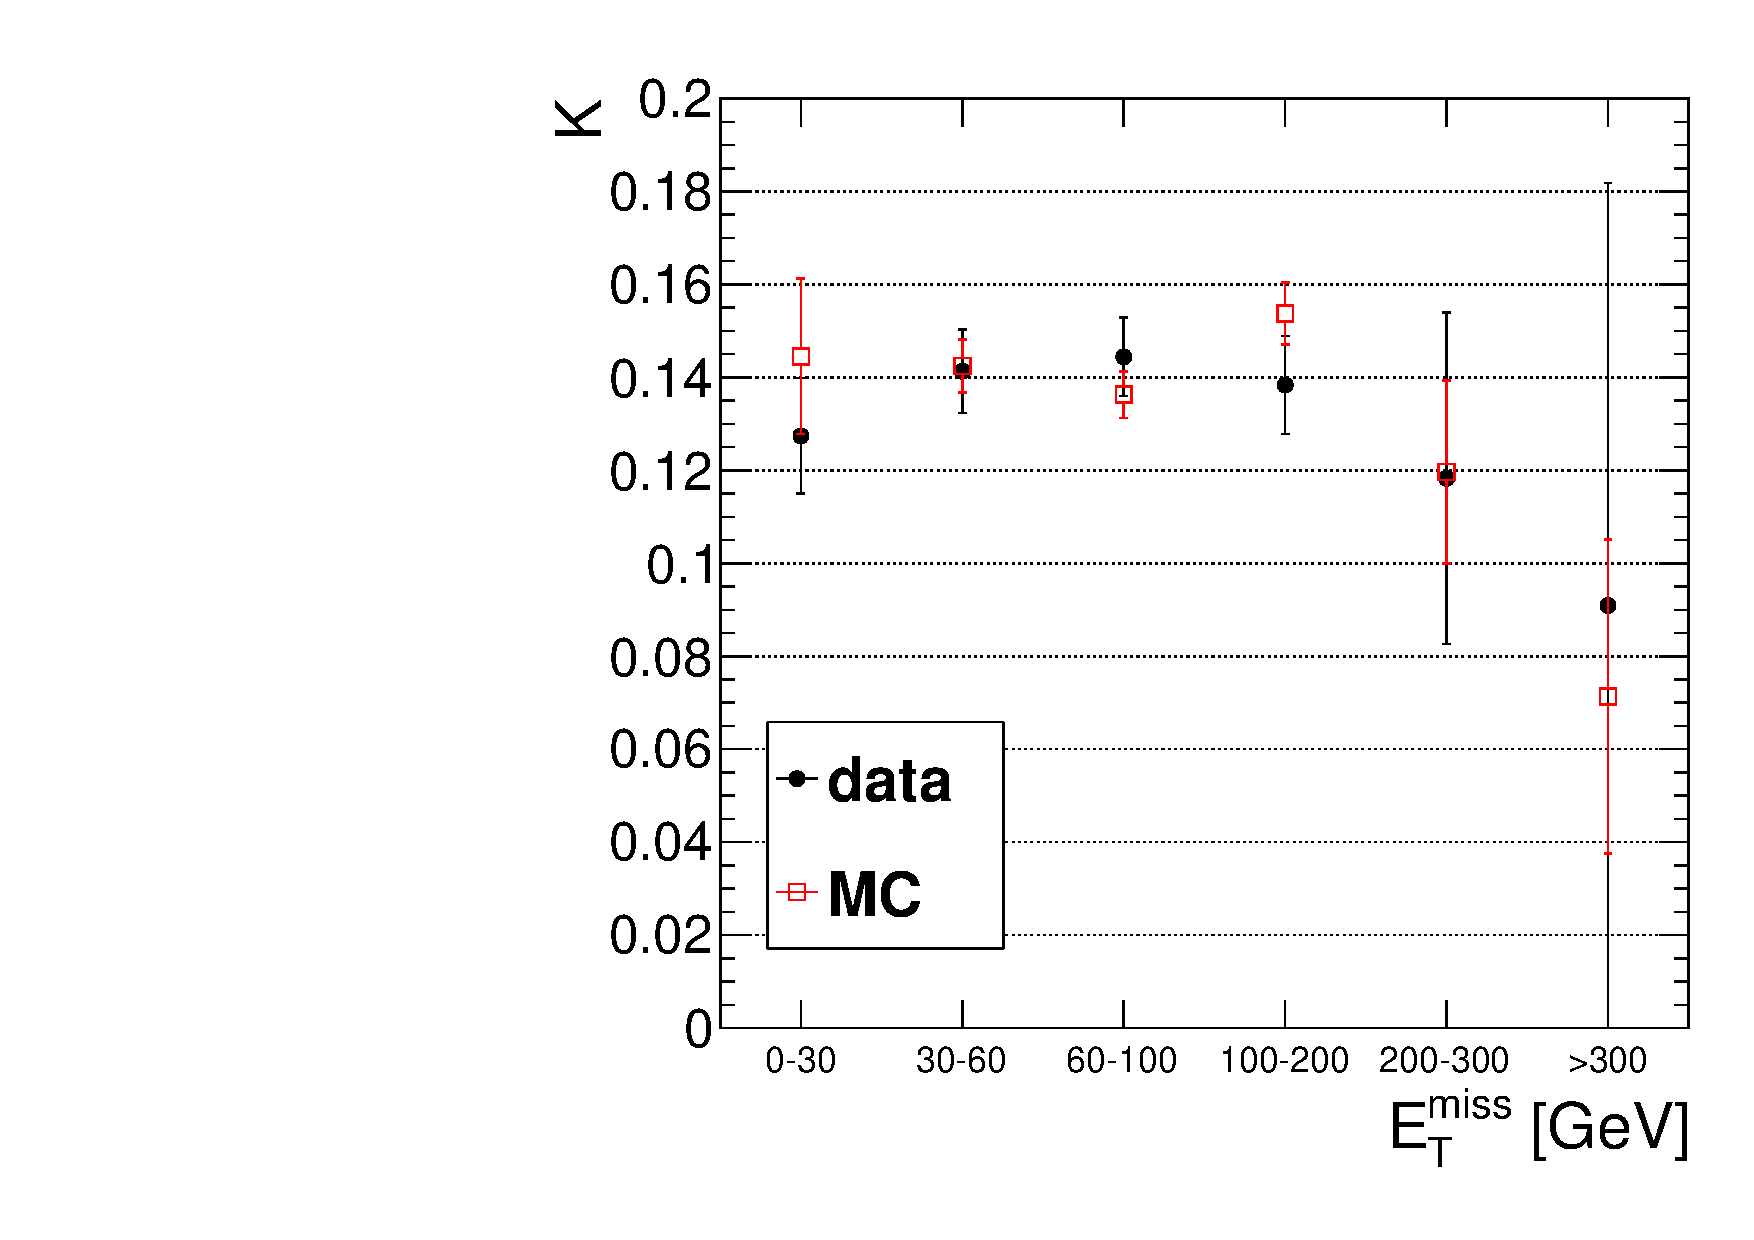
\includegraphics[width=0.4\textwidth]{plots/extractK_exclusive_lowmet.pdf} \\
\end{tabular}
\caption{\label{fig:K_incl_lowmet}
The efficiency for e$\mu$ events to satisfy the dilepton mass requirement, $K$, in data and simulation for inclusive \MET\ intervals 
(left) and exclusive \MET\ intervals (right) for the dilepton \pt\ $>$ (20,20) GeV selection with at least 3 \pt\ $>$ 40 GeV jets
(used for the low \MET\ signal region). 
}
\end{center}
\end{figure}

\begin{comment}

Using selection : ((((leptype==2)&&(csc==0 && hbhe==1 && hcallaser==1 && ecaltp==1 && trkfail==1 && eebadsc==1 && hbhenew==1))&&(isdata==0 || (run<197556 || run>198913)))&&(njets40>=3))&&(lep1.pt()>20 && lep2.pt()>20)
Using weight    : vtxweight * weight
OF entries (total)  5934
OF entries (Z mass) 827
K                   0.139366

--------------------------------------------------------------
pfmet>0

data  : 
total : 5934
Z     : 827
K     : 0.14 +/- 0.005

MC    : 
total : 725.106
Z     : 103.443
K     : 0.14 +/- 0.004
--------------------------------------------------------------


--------------------------------------------------------------
pfmet>30

data  : 
total : 5110
Z     : 722
K     : 0.14 +/- 0.005

MC    : 
total : 625.723
Z     : 89.0789
K     : 0.14 +/- 0.003
--------------------------------------------------------------


--------------------------------------------------------------
pfmet>60

data  : 
total : 3362
Z     : 475
K     : 0.14 +/- 0.006

MC    : 
total : 418.375
Z     : 59.5404
K     : 0.14 +/- 0.004
--------------------------------------------------------------


--------------------------------------------------------------
pfmet>100

data  : 
total : 1347
Z     : 184
K     : 0.14 +/- 0.010

MC    : 
total : 177.754
Z     : 26.7455
K     : 0.15 +/- 0.006
--------------------------------------------------------------


--------------------------------------------------------------
pfmet>200

data  : 
total : 104
Z     : 12
K     : 0.12 +/- 0.033

MC    : 
total : 14.1212
Z     : 1.59283
K     : 0.11 +/- 0.018
--------------------------------------------------------------


--------------------------------------------------------------
pfmet>300

data  : 
total : 11
Z     : 1
K     : 0.09 +/- 0.091

MC    : 
total : 2.00086
Z     : 0.142752
K     : 0.07 +/- 0.034
--------------------------------------------------------------

root [3] Info in <TCanvas::Print>: pdf file /home/users/benhoob/ZMet2012/plots/extractK_inclusive_lowmet.pdf has been created

root [3] 
root [3] extractK(true,false,false)
Using selection : ((((leptype==2)&&(csc==0 && hbhe==1 && hcallaser==1 && ecaltp==1 && trkfail==1 && eebadsc==1 && hbhenew==1))&&(isdata==0 || (run<197556 || run>198913)))&&(njets40>=3))&&(lep1.pt()>20 && lep2.pt()>20)
Using weight    : vtxweight * weight
OF entries (total)  5934
OF entries (Z mass) 827
K                   0.139366
Warning in <TFile::Append>: Replacing existing TH1: htot (Potential memory leak).
Warning in <TFile::Append>: Replacing existing TH1: hZ (Potential memory leak).

--------------------------------------------------------------
pfmet>0   && pfmet<30

data  : 
total : 824
Z     : 105
K     : 0.13 +/- 0.012

MC    : 
total : 99.3853
Z     : 14.3649
K     : 0.14 +/- 0.017
--------------------------------------------------------------


--------------------------------------------------------------
pfmet>30  && pfmet<60

data  : 
total : 1748
Z     : 247
K     : 0.14 +/- 0.009

MC    : 
total : 207.368
Z     : 29.5391
K     : 0.14 +/- 0.006
--------------------------------------------------------------


--------------------------------------------------------------
pfmet>60  && pfmet<100

data  : 
total : 2015
Z     : 291
K     : 0.14 +/- 0.008

MC    : 
total : 240.615
Z     : 32.7949
K     : 0.14 +/- 0.005
--------------------------------------------------------------


--------------------------------------------------------------
pfmet>100 && pfmet<200

data  : 
total : 1243
Z     : 172
K     : 0.14 +/- 0.011

MC    : 
total : 163.632
Z     : 25.1526
K     : 0.15 +/- 0.007
--------------------------------------------------------------


--------------------------------------------------------------
pfmet>200 && pfmet<300

data  : 
total : 93
Z     : 11
K     : 0.12 +/- 0.036

MC    : 
total : 12.1203
Z     : 1.45008
K     : 0.12 +/- 0.020
--------------------------------------------------------------


--------------------------------------------------------------
pfmet>300

data  : 
total : 11
Z     : 1
K     : 0.09 +/- 0.091

MC    : 
total : 2.00086
Z     : 0.142752
K     : 0.07 +/- 0.034
--------------------------------------------------------------


\end{comment}

\subsection{Results in Z Mass Window}

The results of the low \MET\ signal region are displayed in Fig.~\ref{fig:results_lowmet} and summarized in Table~\ref{tab:results_lowmet},
separately for the Run2012A+B data (5.1 fb$^{-1}$) and Run2012C data (4.1 fb$^{-1}$).
In the Run2012A+B data, we observed a 1.6$\sigma$ excess for \MET\ $>$ 100 GeV, corresponding to the low \MET\ signal region.
However, this excess does not persist in Run2012C data, where we observe good agreement between the data and the predicted background.
In the combined Run2012A+B+C data (Fig.~\ref{fig:results_fulledge} and Table~\ref{tab:results_edgefull}) we observe reasonable
agreement over the full \MET\ range. In the \MET\ $>$ 100 GeV region we observe 288 events with a predicted background of $251\pm33$,
representing an excess of 1.0$\sigma$.

The results of the high \MET\ signal region are displayed in Fig.~\ref{fig:results_highmet} and summarized in 
Table~\ref{tab:results_highmet},
separately for the Run2012A+B data (5.1 fb$^{-1}$) and Run2012C data (4.1 fb$^{-1}$).
In both periods we observe good agreement between the data and predicted background over the full \MET\ range.
In the combined Run2012A+B+C data (Fig.~\ref{fig:results_fulledge} and Table~\ref{tab:results_edgefull}) we observe reasonable
agreement over the full \MET\ range. 
In the \MET\ $>$ 150 GeV region corresponding to the high \MET\ signal region in the full sample, we observe 167 events with a predicted
background of $177\pm25$ events, representing a deficit of -0.4$\sigma$.

\clearpage

\begin{figure}[!h]
\begin{center}
\begin{tabular}{cc}
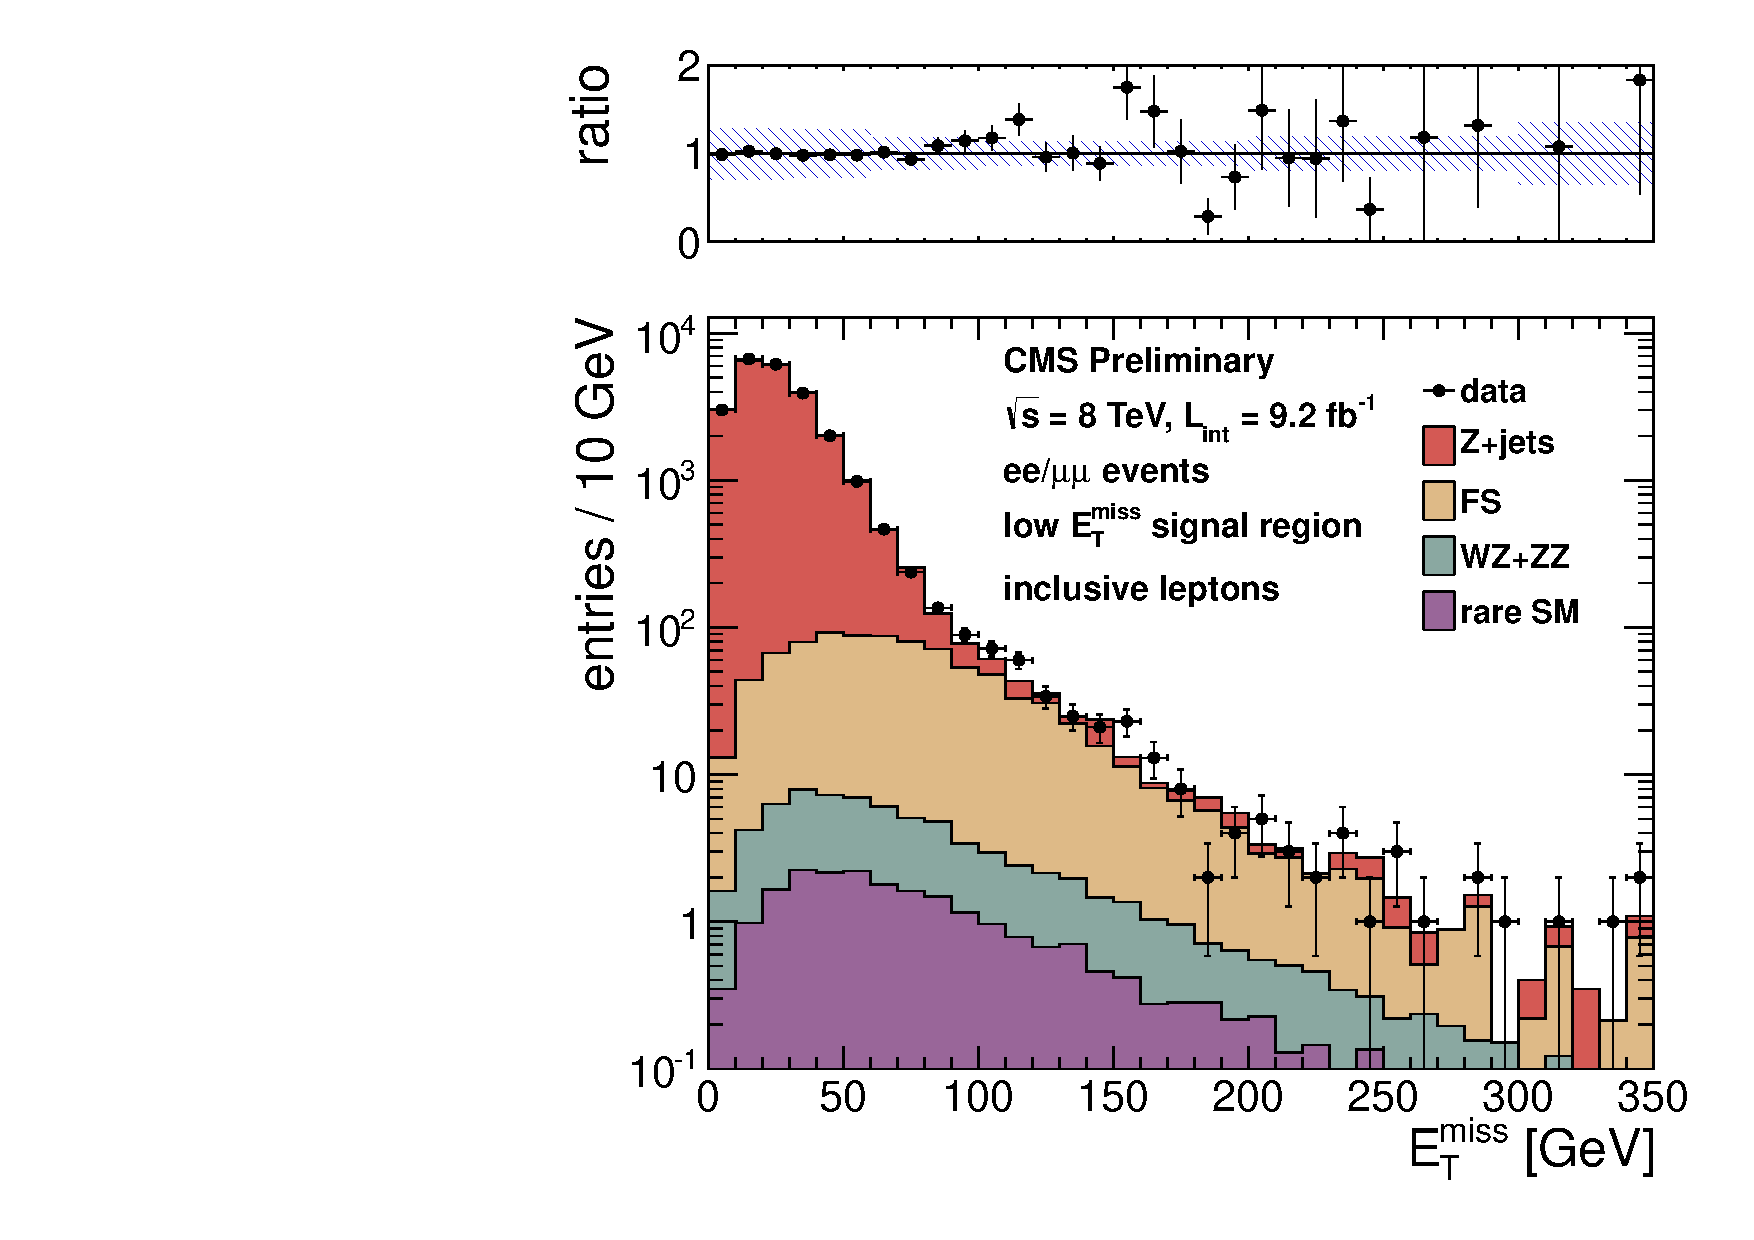
\includegraphics[width=0.45\textwidth]{plots/edge_pfmet_pt40_lowMet_all.pdf}
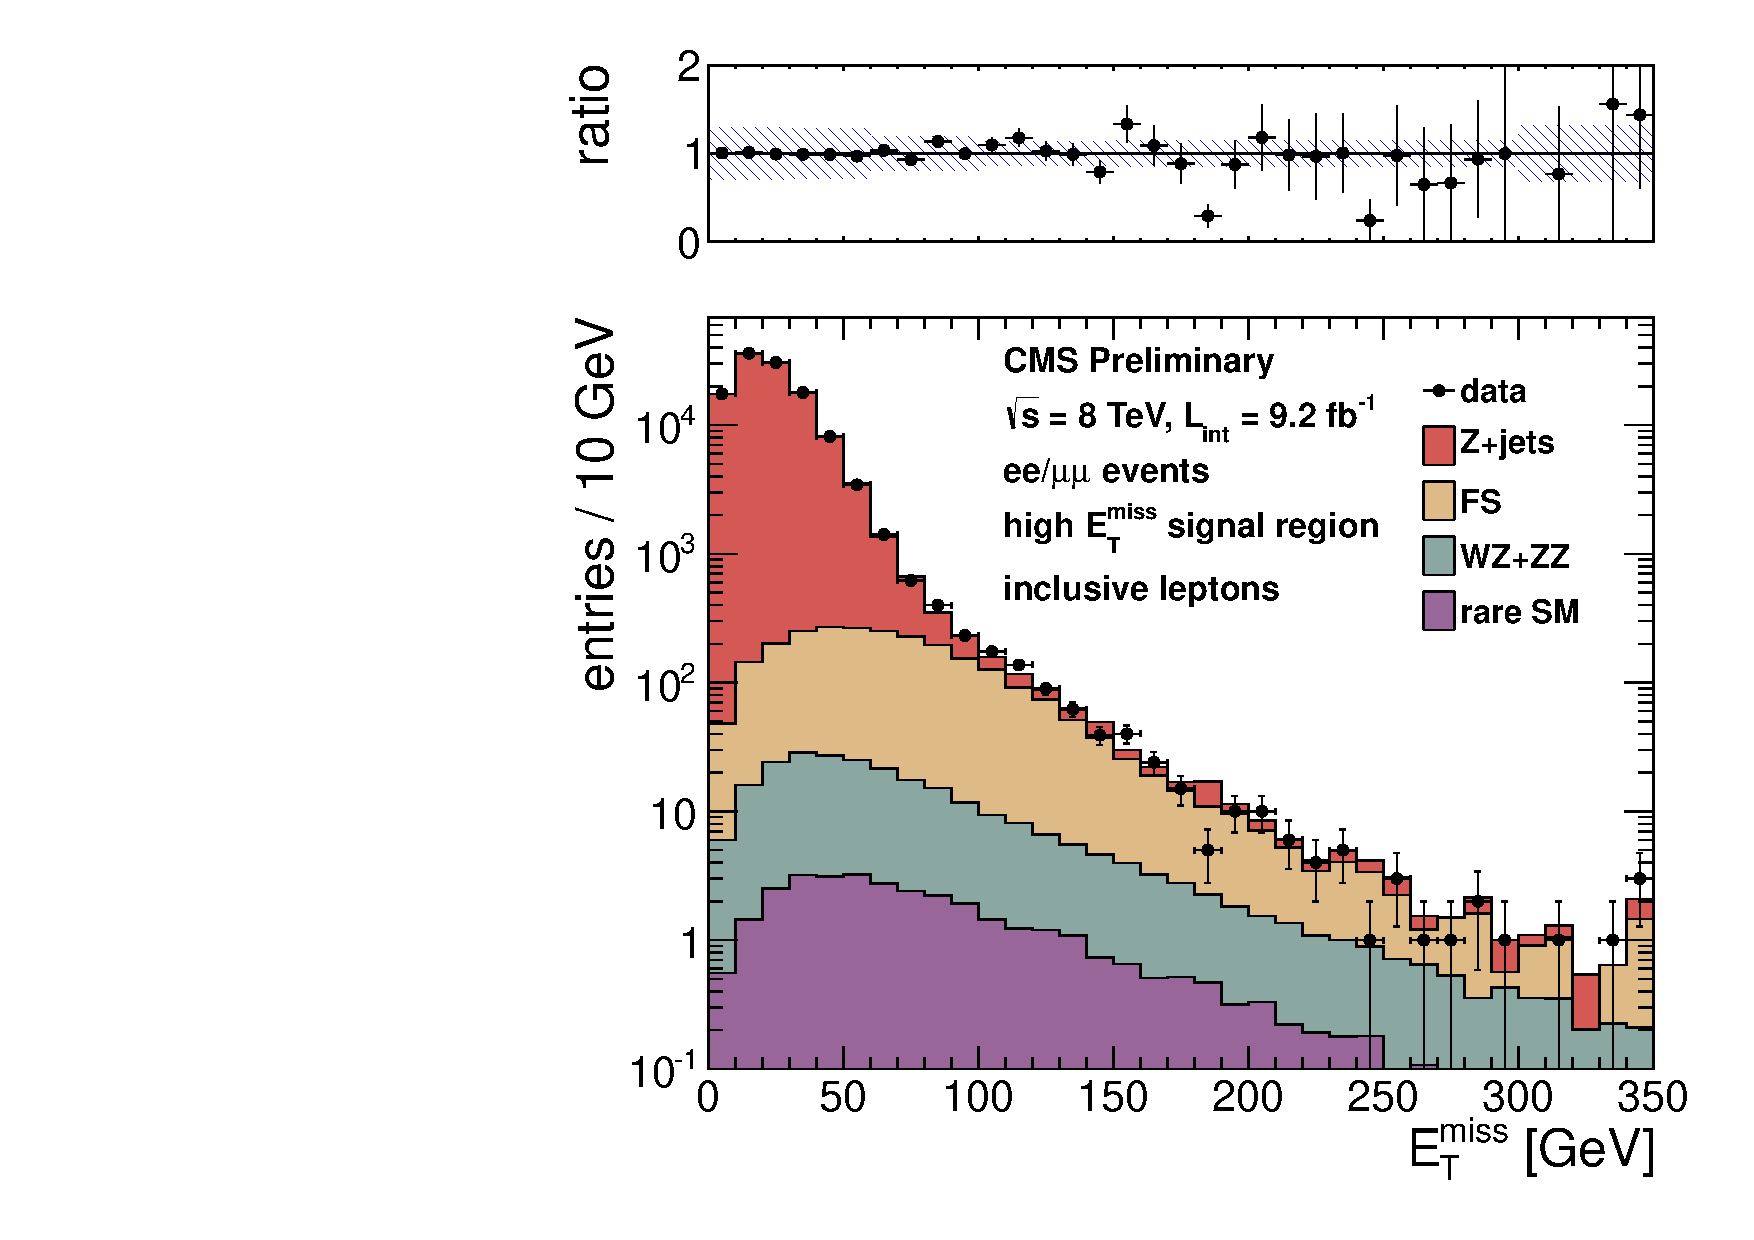
\includegraphics[width=0.45\textwidth]{plots/edge_pfmet_pt40_highMet_all.pdf}
%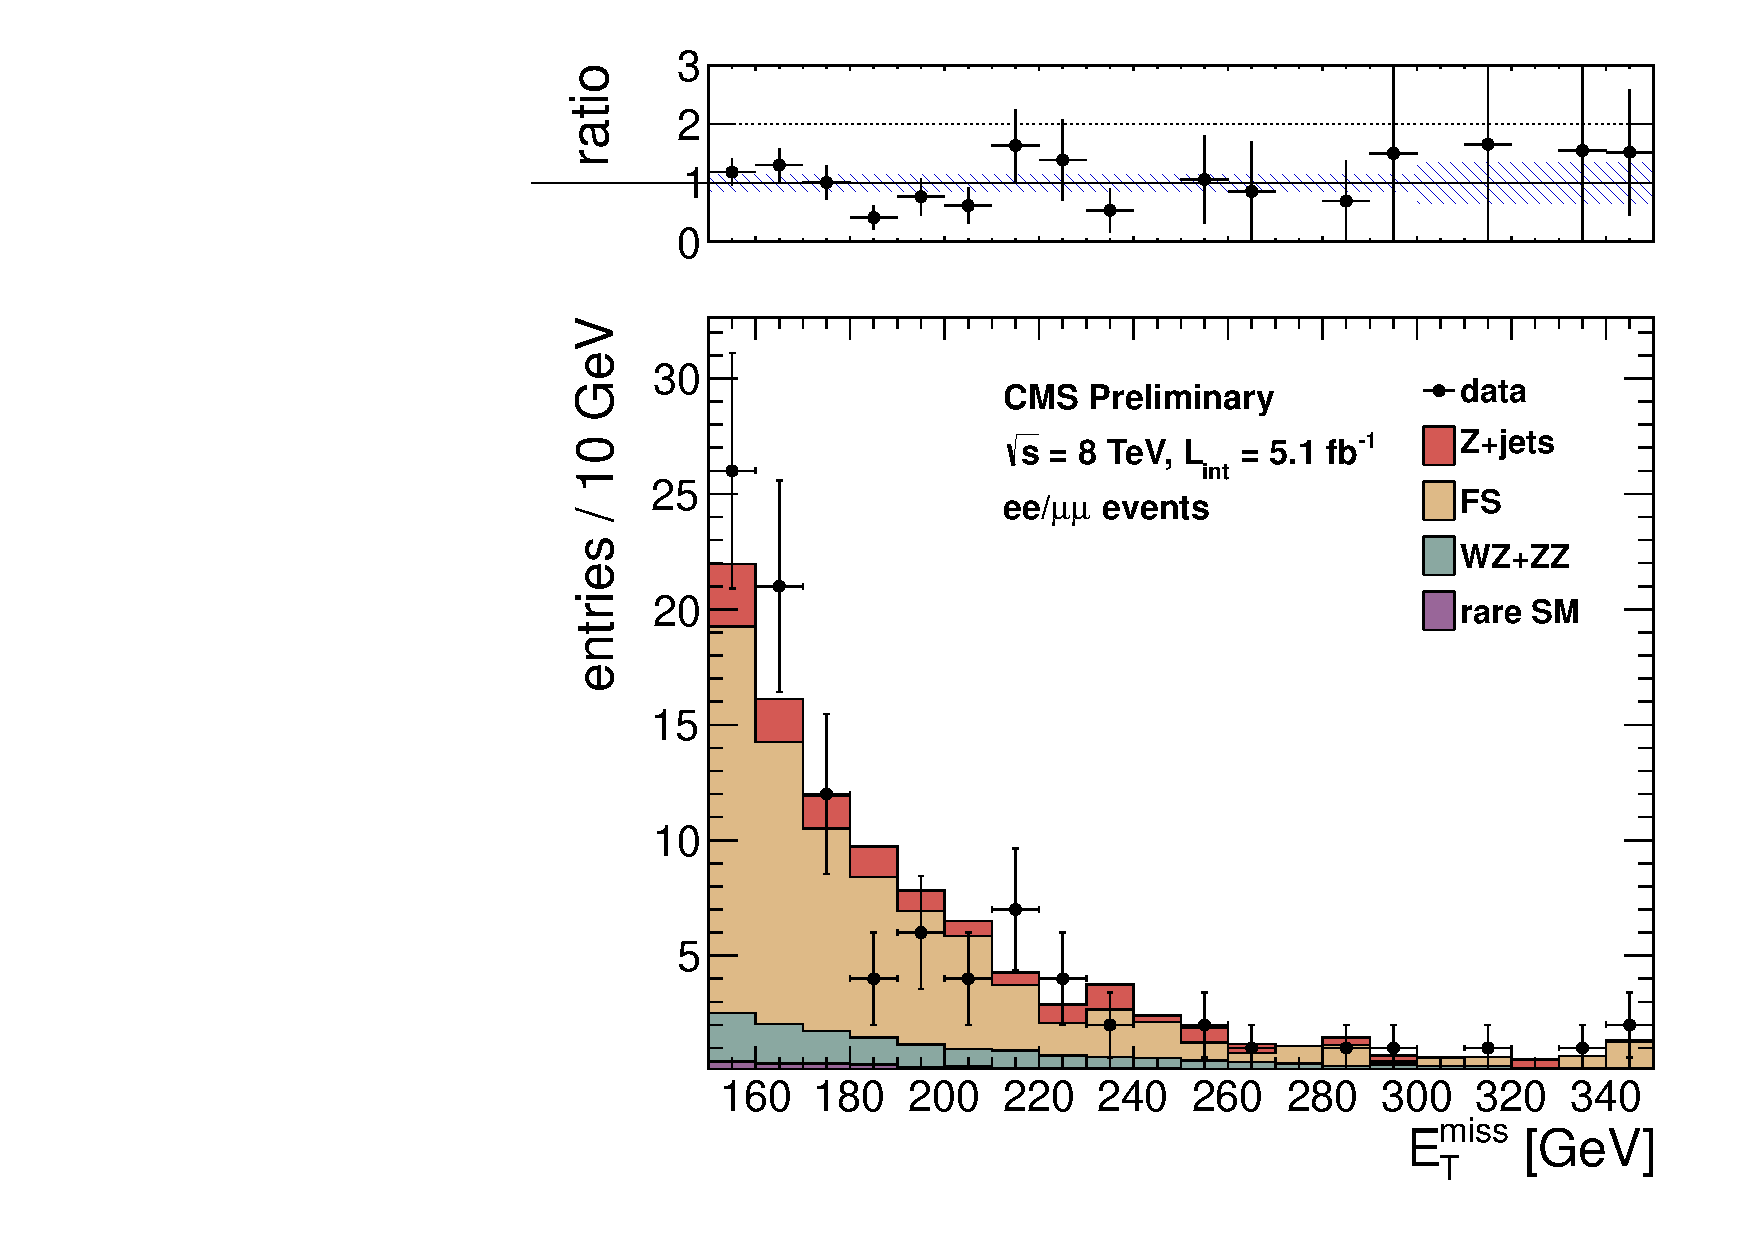
\includegraphics[width=0.48\textwidth]{plots/pfmet_pt40_2012AB_highMet_all_linear.pdf}
\end{tabular}
\caption{\footnotesize {\bf Results of for the low \MET\ (left) and high \MET\ (right) signal regions with the inclusive lepton selection.}
The observed \MET\ distribution (black points) is compared with the sum of the predicted \MET\
distributions from \zjets, flavor-symmetric backgrounds, WZ+ZZ backgrounds, and rare SM backgrounds. 
The ratio of observed to predicted yields in each bin is
indicated. The error bars indicate the statistical uncertainty in the data and the shaded band indicates the total background uncertainty.
\label{fig:results_fulledge}
}
\end{center}
\end{figure}

\begin{table}[htb]
\begin{center}
\footnotesize
\caption{\label{tab:results_edgefull}\footnotesize {\bf Results for the low \MET\ signal region (top table) and high \MET\ signal region (bottom table) with the inclusive lepton selection.} 
The total background is the sum of the \zjets\ background predicted from
the \MET\ templates method (\zjets\ bkg), the flavor-symmetric background predicted from e$\mu$ events (FS bkg), the WZ and ZZ backgrounds predicted from MC
(WZ bkg and ZZ bkg) and the rare SM backgrounds. All uncertainties include both the statistical and systematic components. The Gaussian significance of the deviation between the data 
and total background is indicated for signal regions with at least 20 observed events. }
\begin{tabular}{l|c|c|c|c|c|c}

\hline
\hline

\begin{comment}
Using pfmet out-of-the-box
NEED TO RE-EVALUATE K!!!!!!!!!!!!!!!!!
Using pT > 40 GeV jets, low MET signal region
WZ/ZZ selection : ((((((leptype==0 && (ee==1 || isdata==0))||(leptype==1 && (mm==1 || isdata==0)))&&(ngennu>0))&&(csc==0 && hbhe==1 && hcallaser==1 && ecaltp==1 && trkfail==1 && eebadsc==1 && hbhenew==1))&&(dilmass>81 && dilmass<101))&&(lep1.pt()>20.0 && lep2.pt()>20.0))&&(njets40>=3)
WZ/ZZ weight    : weight * 9.2 * vtxweight * trgeff
Opening ../output/V00-01-04/babylooper_edge_data_ALL_53X_PhotonStitchedTemplate_pfmet_pt40_lowMet.root
B-veto?   0
K         0.14
ee+mm channels: scale em yield by 0.99
Yields in 0-60 GeV region
data   : 22782
gjets  : 23299
OF     : 350.242
WZ     : 22.2641
ZZ     : 2.36791
Rare   : 9.60548
Scaling gjets by : 0.961309
SF events 23999
OF events 5826

ee/#mu#mu events
\end{comment}


                      &   \MET\ $>$ 0 GeV   &  \MET\ $>$ 30 GeV   &  \MET\ $>$ 60 GeV   & \MET\ $>$ 100 GeV   & \MET\ $>$ 200 GeV   & \MET\ $>$ 300 GeV  \\
\hline
        \zjets\ bkg   &  23071 $\pm$ 6922   &   7456 $\pm$ 2238   &     673 $\pm$ 203   &   49.9 $\pm$ 16.4   &     4.4 $\pm$ 1.8   &     1.0 $\pm$ 0.6  \\
             FS bkg   &     807 $\pm$ 126   &     695 $\pm$ 108   &      457 $\pm$ 71   &      184 $\pm$ 29   &    14.1 $\pm$ 3.4   &     1.5 $\pm$ 0.9  \\
             WZ bkg   &   43.5 $\pm$ 30.5   &   35.1 $\pm$ 24.6   &   21.3 $\pm$ 14.9   &    10.0 $\pm$ 7.1   &     1.9 $\pm$ 1.7   &     0.4 $\pm$ 0.4  \\
             ZZ bkg   &     7.8 $\pm$ 3.9   &     7.0 $\pm$ 3.6   &     5.4 $\pm$ 2.8   &     3.3 $\pm$ 1.8   &     0.9 $\pm$ 0.8   &     0.2 $\pm$ 0.2  \\
        rare SM bkg   &   22.0 $\pm$ 11.0   &    19.0 $\pm$ 9.6   &    12.4 $\pm$ 6.3   &     6.3 $\pm$ 3.3   &     1.3 $\pm$ 1.1   &     0.3 $\pm$ 0.3  \\
\hline
          total bkg   &  23951 $\pm$ 6924   &   8213 $\pm$ 2241   &    1169 $\pm$ 216   &      253 $\pm$ 34   &    22.6 $\pm$ 4.4   &     3.5 $\pm$ 1.2  \\
               data   &             23999   &              8134   &              1217   &               288   &                26   &                 4  \\
       significance   &       0.0$\sigma$   &      -0.0$\sigma$   &       0.2$\sigma$   &       0.9$\sigma$   &       0.5$\sigma$   &                    \\
\hline
\hline


\begin{comment}
Using pfmet out-of-the-box
NEED TO RE-EVALUATE K!!!!!!!!!!!!!!!!!
Using pT > 40 GeV jets, high MET signal region
WZ/ZZ selection : (((((((leptype==0 && (ee==1 || isdata==0))||(leptype==1 && (mm==1 || isdata==0)))&&(ngennu>0))&&(csc==0 && hbhe==1 && hcallaser==1 && ecaltp==1 && trkfail==1 && eebadsc==1 && hbhenew==1))&&(dilmass>81 && dilmass<101))&&(lep1.pt()>20.0 && lep2.pt()>20.0))&&(njets40>=2))&&(ht40>=100.0)
WZ/ZZ weight    : weight * 9.2 * vtxweight * trgeff
Opening ../output/V00-01-04/babylooper_edge_data_ALL_53X_PhotonStitchedTemplate_pfmet_pt40_highMet.root
B-veto?   0
K         0.14
ee+mm channels: scale em yield by 0.99
Yields in 0-60 GeV region
data   : 113677
gjets  : 115027
OF     : 1054.05
WZ     : 100.866
ZZ     : 11.955
Rare   : 14.0179
Scaling gjets by : 0.978
SF events 116978
OF events 16270

ee/#mu#mu events
\end{comment}

                      &   \MET\ $>$ 0 GeV   &  \MET\ $>$ 30 GeV   &  \MET\ $>$ 60 GeV   & \MET\ $>$ 100 GeV   & \MET\ $>$ 150 GeV   & \MET\ $>$ 300 GeV  \\
\hline
        \zjets\ bkg   &114401 $\pm$ 34322   &  30966 $\pm$ 9291   &    1905 $\pm$ 573   &      120 $\pm$ 38   &    26.2 $\pm$ 8.9   &     1.4 $\pm$ 0.7  \\
             FS bkg   &    2255 $\pm$ 373   &    1908 $\pm$ 316   &    1201 $\pm$ 199   &      436 $\pm$ 72   &   90.0 $\pm$ 15.3   &     2.9 $\pm$ 1.3  \\
             WZ bkg   & 182.7 $\pm$ 127.9   & 144.7 $\pm$ 101.3   &   81.8 $\pm$ 57.3   &   35.2 $\pm$ 24.7   &    13.9 $\pm$ 9.9   &     1.3 $\pm$ 1.3  \\
             ZZ bkg   &   35.9 $\pm$ 18.0   &   32.3 $\pm$ 16.2   &   23.9 $\pm$ 12.0   &    14.0 $\pm$ 7.1   &     6.7 $\pm$ 3.6   &     0.8 $\pm$ 0.8  \\
        rare SM bkg   &   33.5 $\pm$ 16.8   &   29.0 $\pm$ 14.6   &    19.5 $\pm$ 9.8   &    10.2 $\pm$ 5.2   &     4.5 $\pm$ 2.5   &     0.5 $\pm$ 0.5  \\
\hline
          total bkg   &116908 $\pm$ 34324   &  33080 $\pm$ 9297   &    3231 $\pm$ 609   &      616 $\pm$ 86   &      141 $\pm$ 21   &     6.9 $\pm$ 2.2  \\
               data   &            116978   &             32796   &              3301   &               635   &               133   &                 5  \\
       significance   &       0.0$\sigma$   &      -0.0$\sigma$   &       0.1$\sigma$   &       0.2$\sigma$   &      -0.4$\sigma$   &      -0.6$\sigma$  \\
\hline
\hline

\end{tabular}
\end{center}
\end{table}

\clearpage


\begin{figure}[!h]
\begin{center}
\begin{tabular}{cc}
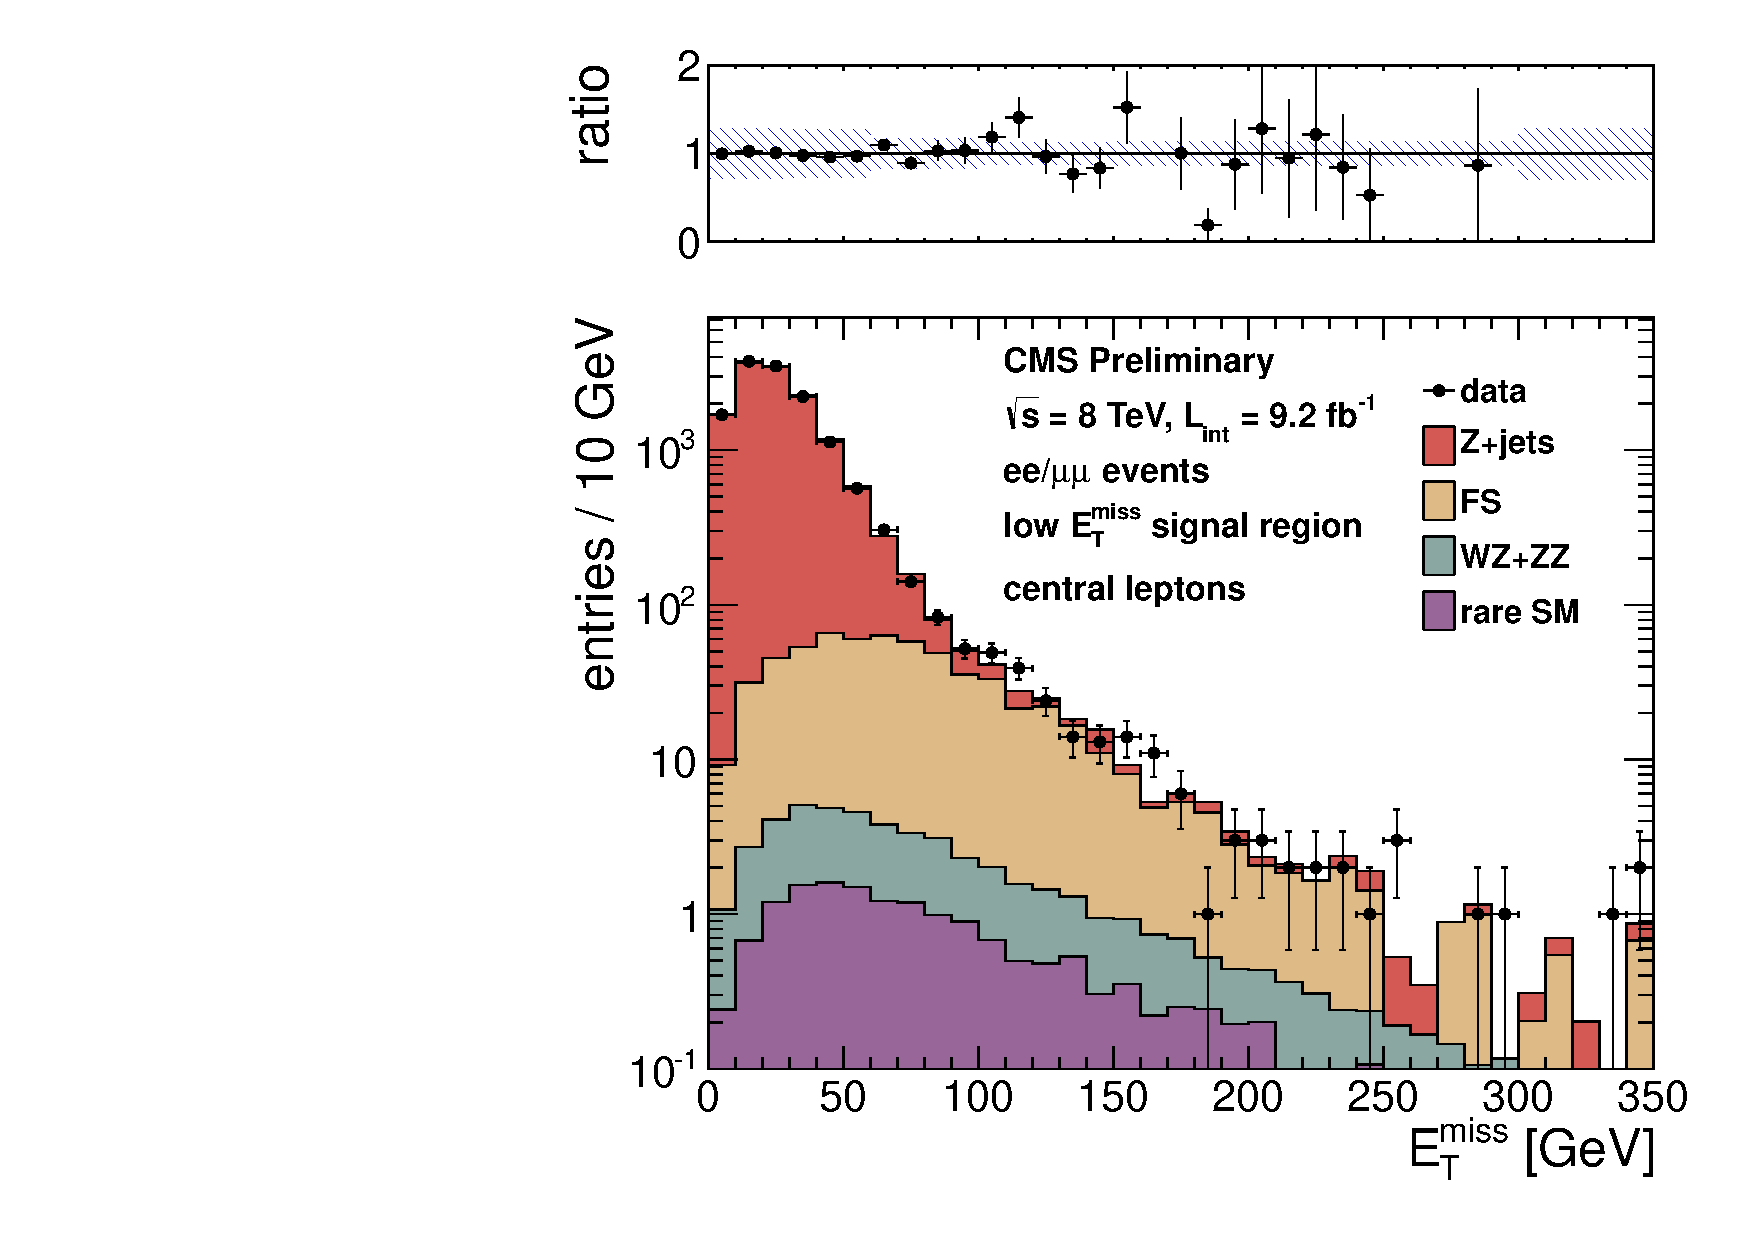
\includegraphics[width=0.45\textwidth]{plots/edge_pfmet_pt40_lowMet_central_all.pdf}
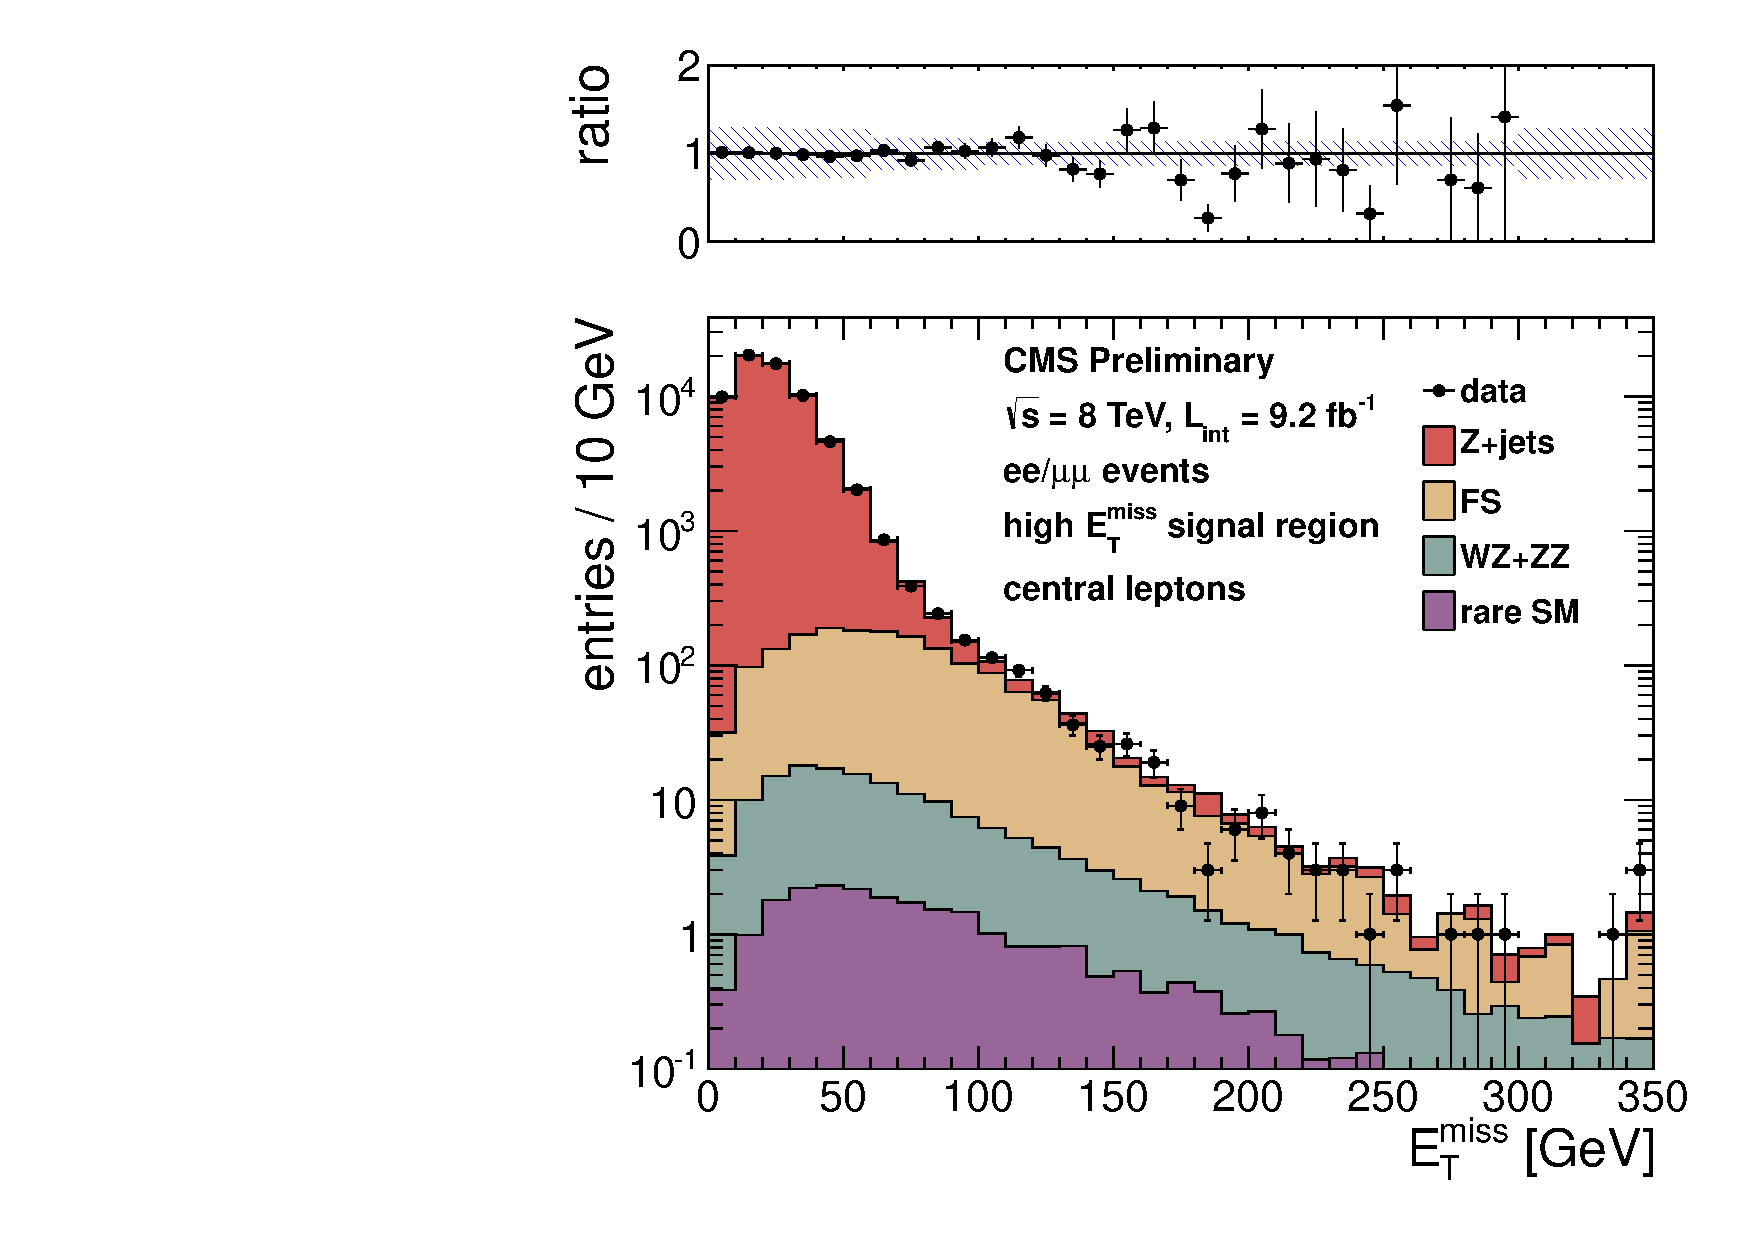
\includegraphics[width=0.45\textwidth]{plots/edge_pfmet_pt40_highMet_central_all.pdf}
%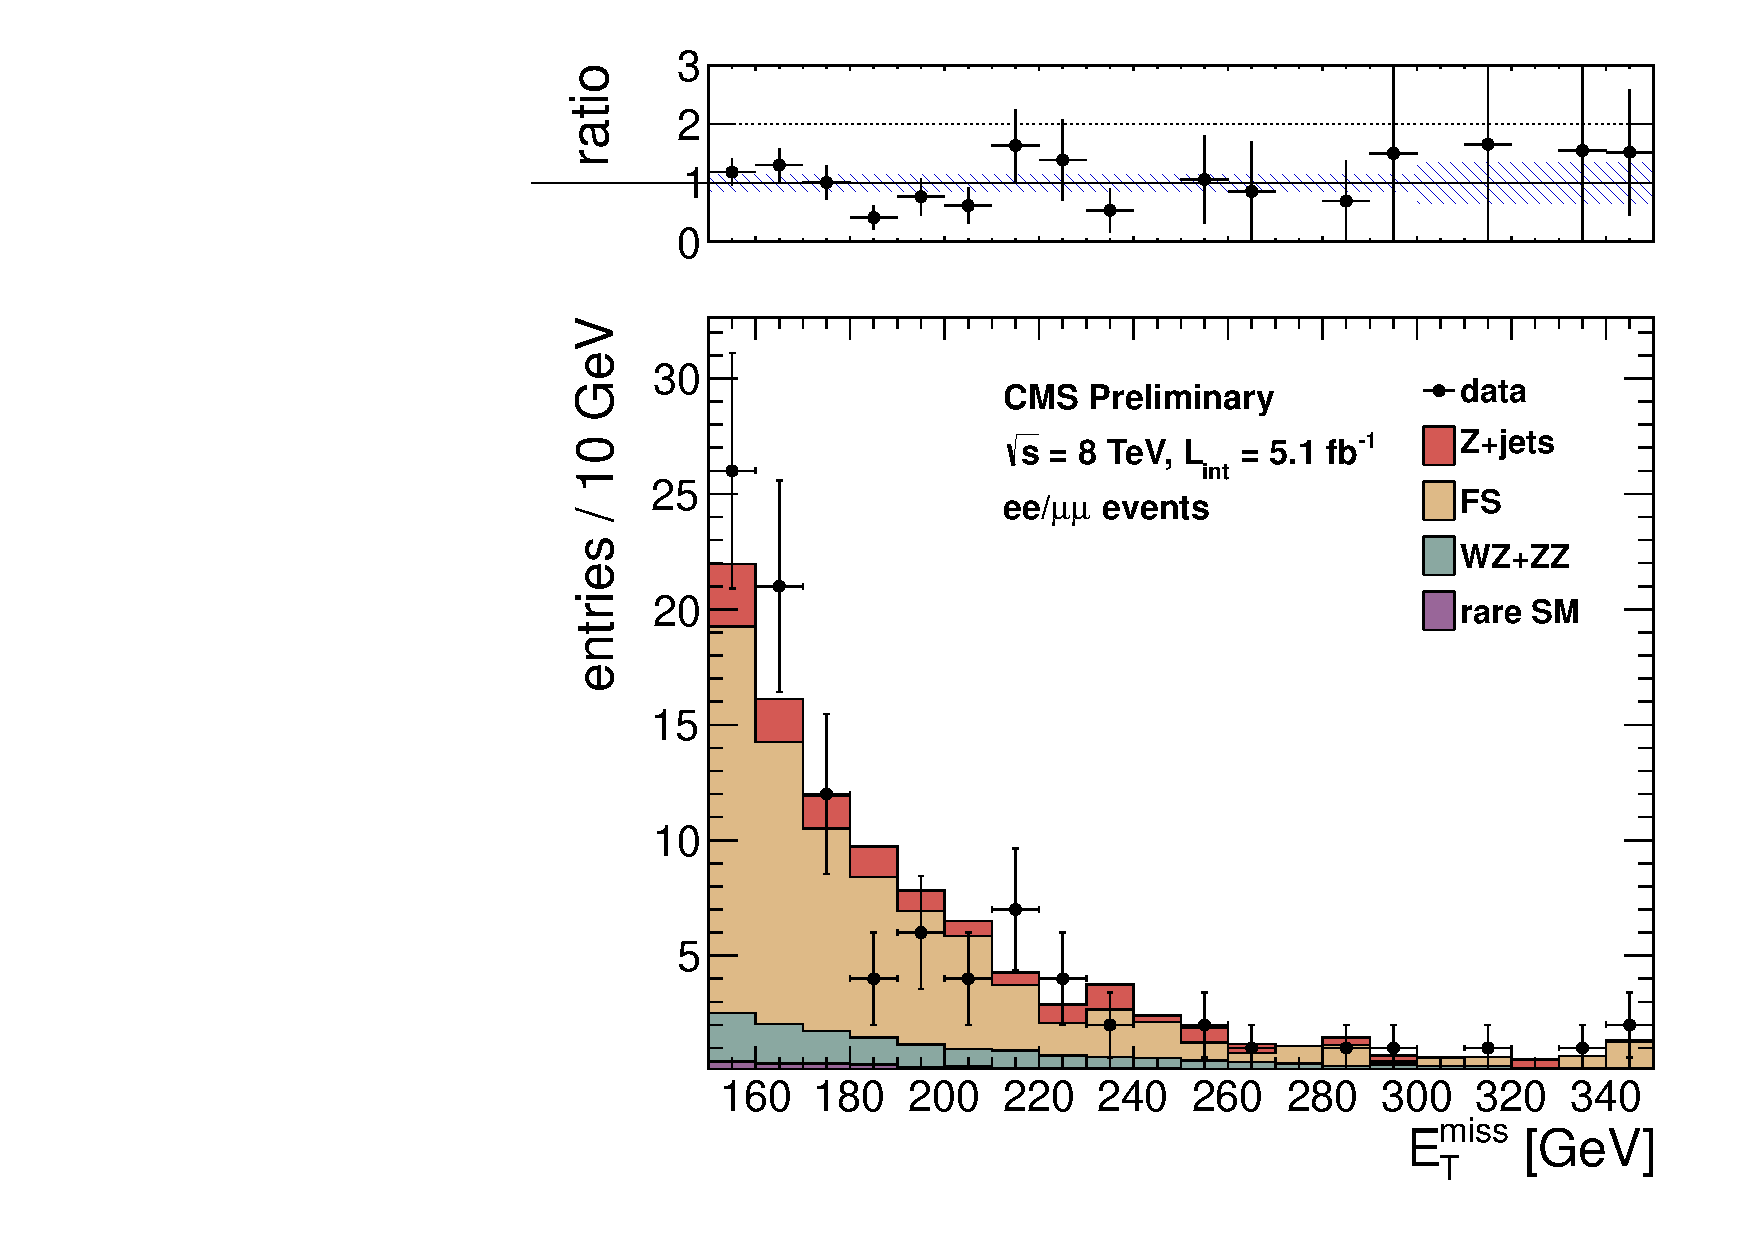
\includegraphics[width=0.48\textwidth]{plots/pfmet_pt40_2012AB_highMet_all_linear.pdf}
\end{tabular}
\caption{\footnotesize {\bf Results of for the low \MET\ (left) and high \MET\ (right) signal regions with the central lepton selection.}
The observed \MET\ distribution (black points) is compared with the sum of the predicted \MET\
distributions from \zjets, flavor-symmetric backgrounds, WZ+ZZ backgrounds, and rare SM backgrounds. 
The ratio of observed to predicted yields in each bin is
indicated. The error bars indicate the statistical uncertainty in the data and the shaded band indicates the total background uncertainty.
\label{fig:results_fulledge_central}
}
\end{center}
\end{figure}

\begin{table}[htb]
\begin{center}
\footnotesize
\caption{\label{tab:results_edgefull_central}\footnotesize {\bf Results for the low \MET\ signal region (top table) and high \MET\ signal region (bottom table) with the central lepton selection.} 
The total background is the sum of the \zjets\ background predicted from
the \MET\ templates method (\zjets\ bkg), the flavor-symmetric background predicted from e$\mu$ events (FS bkg), the WZ and ZZ backgrounds predicted from MC
(WZ bkg and ZZ bkg) and the rare SM backgrounds. All uncertainties include both the statistical and systematic components. The Gaussian significance of the deviation between the data 
and total background is indicated for signal regions with at least 20 observed events. }
\begin{tabular}{l|c|c|c|c|c|c}

\hline
\hline

\begin{comment}
Using pfmet out-of-the-box
NEED TO RE-EVALUATE K!!!!!!!!!!!!!!!!!
Using pT > 40 GeV jets, low MET signal region, central leptons
WZ/ZZ selection : (((((((leptype==0 && (ee==1 || isdata==0))||(leptype==1 && (mm==1 || isdata==0)))&&(ngennu>0))&&(csc==0 && hbhe==1 && hcallaser==1 && ecaltp==1 && trkfail==1 && eebadsc==1 && hbhenew==1))&&(dilmass>81 && dilmass<101))&&(lep1.pt()>20.0 && lep2.pt()>20.0))&&(njets40>=3))&&(abs(lep1.eta()) < 1.4 && abs(lep2.eta()) < 1.4)
WZ/ZZ weight    : weight * 9.2 * vtxweight * trgeff
Opening ../output/V00-01-04/babylooper_edge_data_ALL_53X_PhotonStitchedTemplate_pfmet_pt40_lowMet_central.root
B-veto?   0
K         0.14
ee+mm channels: scale em yield by 0.99
Yields in 0-60 GeV region
data   : 12858
gjets  : 13220.3
OF     : 226.472
WZ     : 14.1734
ZZ     : 1.45279
Rare   : 6.75969
Scaling gjets by : 0.953773
SF events 13631
OF events 3806

ee/#mu#mu events
\end{comment}

                      &   \MET\ $>$ 0 GeV   &  \MET\ $>$ 30 GeV   &  \MET\ $>$ 60 GeV   & \MET\ $>$ 100 GeV   & \MET\ $>$ 200 GeV   & \MET\ $>$ 300 GeV  \\
\hline
        \zjets\ bkg   &  13001 $\pm$ 3901   &   4247 $\pm$ 1275   &     392 $\pm$ 118   &    29.7 $\pm$ 9.7   &     2.6 $\pm$ 1.1   &     0.6 $\pm$ 0.4  \\
             FS bkg   &      528 $\pm$ 82   &      455 $\pm$ 71   &      301 $\pm$ 47   &      121 $\pm$ 19   &     9.6 $\pm$ 2.4   &     1.1 $\pm$ 0.7  \\
             WZ bkg   &   28.1 $\pm$ 19.7   &   22.7 $\pm$ 15.9   &    13.9 $\pm$ 9.8   &     6.8 $\pm$ 4.9   &     1.5 $\pm$ 1.4   &     0.4 $\pm$ 0.4  \\
             ZZ bkg   &     4.8 $\pm$ 2.5   &     4.4 $\pm$ 2.3   &     3.3 $\pm$ 1.8   &     2.1 $\pm$ 1.2   &     0.6 $\pm$ 0.6   &     0.1 $\pm$ 0.1  \\
        rare SM bkg   &    15.8 $\pm$ 8.0   &    13.7 $\pm$ 6.9   &     9.0 $\pm$ 4.6   &     4.8 $\pm$ 2.5   &     1.0 $\pm$ 1.0   &     0.3 $\pm$ 0.3  \\
\hline
          total bkg   &  13577 $\pm$ 3902   &   4743 $\pm$ 1277   &     719 $\pm$ 128   &      164 $\pm$ 22   &    15.3 $\pm$ 3.2   &     2.5 $\pm$ 0.9  \\
               data   &             13631   &              4688   &               773   &               192   &                18   &                 3  \\
       significance   &       0.0$\sigma$   &      -0.0$\sigma$   &       0.4$\sigma$   &       1.1$\sigma$   &       0.5$\sigma$   &       0.3$\sigma$  \\



\hline
\hline

\begin{comment}
Using pfmet out-of-the-box
NEED TO RE-EVALUATE K!!!!!!!!!!!!!!!!!
Using pT > 40 GeV jets, high MET signal region, central leptons
WZ/ZZ selection : ((((((((leptype==0 && (ee==1 || isdata==0))||(leptype==1 && (mm==1 || isdata==0)))&&(ngennu>0))&&(csc==0 && hbhe==1 && hcallaser==1 && ecaltp==1 && trkfail==1 && eebadsc==1 && hbhenew==1))&&(dilmass>81 && dilmass<101))&&(lep1.pt()>20.0 && lep2.pt()>20.0))&&(njets40>=2))&&(ht40>=100.0))&&(abs(lep1.eta()) < 1.4 && abs(lep2.eta()) < 1.4)
WZ/ZZ weight    : weight * 9.2 * vtxweight * trgeff
Opening ../output/V00-01-04/babylooper_edge_data_ALL_53X_PhotonStitchedTemplate_pfmet_pt40_highMet_central.root
B-veto?   0
K         0.14
ee+mm channels: scale em yield by 0.99
Yields in 0-60 GeV region
data   : 64459
gjets  : 65372.5
OF     : 674.705
WZ     : 62.6465
ZZ     : 6.86106
Rare   : 9.85893
Scaling gjets by : 0.974492
SF events 66521
OF events 10593

ee/#mu#mu events
\end{comment}

                      &   \MET\ $>$ 0 GeV   &  \MET\ $>$ 30 GeV   &  \MET\ $>$ 60 GeV   & \MET\ $>$ 100 GeV   & \MET\ $>$ 150 GeV   & \MET\ $>$ 300 GeV  \\
\hline
        \zjets\ bkg   & 64824 $\pm$ 19448   &  17710 $\pm$ 5314   &    1119 $\pm$ 336   &   71.9 $\pm$ 22.4   &    15.8 $\pm$ 5.3   &     0.8 $\pm$ 0.4  \\
             FS bkg   &    1468 $\pm$ 243   &    1252 $\pm$ 207   &     793 $\pm$ 131   &      292 $\pm$ 49   &   62.1 $\pm$ 10.7   &     2.1 $\pm$ 1.0  \\
             WZ bkg   &  115.0 $\pm$ 80.5   &   91.3 $\pm$ 64.0   &   52.4 $\pm$ 36.7   &   23.3 $\pm$ 16.4   &     9.4 $\pm$ 6.7   &     1.0 $\pm$ 1.0  \\
             ZZ bkg   &   21.7 $\pm$ 10.9   &    19.7 $\pm$ 9.9   &    14.8 $\pm$ 7.5   &     8.8 $\pm$ 4.5   &     4.3 $\pm$ 2.4   &     0.5 $\pm$ 0.5  \\
        rare SM bkg   &   23.9 $\pm$ 12.0   &   20.8 $\pm$ 10.4   &    14.1 $\pm$ 7.1   &     7.5 $\pm$ 3.9   &     3.6 $\pm$ 2.1   &     0.5 $\pm$ 0.5  \\
\hline
          total bkg   & 66453 $\pm$ 19450   &  19094 $\pm$ 5318   &    1994 $\pm$ 363   &      403 $\pm$ 56   &   95.2 $\pm$ 14.1   &     4.9 $\pm$ 1.6  \\
               data   &             66521   &             18841   &              2062   &               421   &                92   &                 4  \\
       significance   &       0.0$\sigma$   &      -0.0$\sigma$   &       0.2$\sigma$   &       0.3$\sigma$   &      -0.2$\sigma$   &      -0.4$\sigma$  \\

\hline
\hline


\end{tabular}
\end{center}
\end{table}

\clearpage


\subsection{Extrapolation to Low Mass to Estimate the $\gamma^*/Z$ Contribution}

\begin{figure}[t]
\begin{center}
\begin{tabular}{cc}
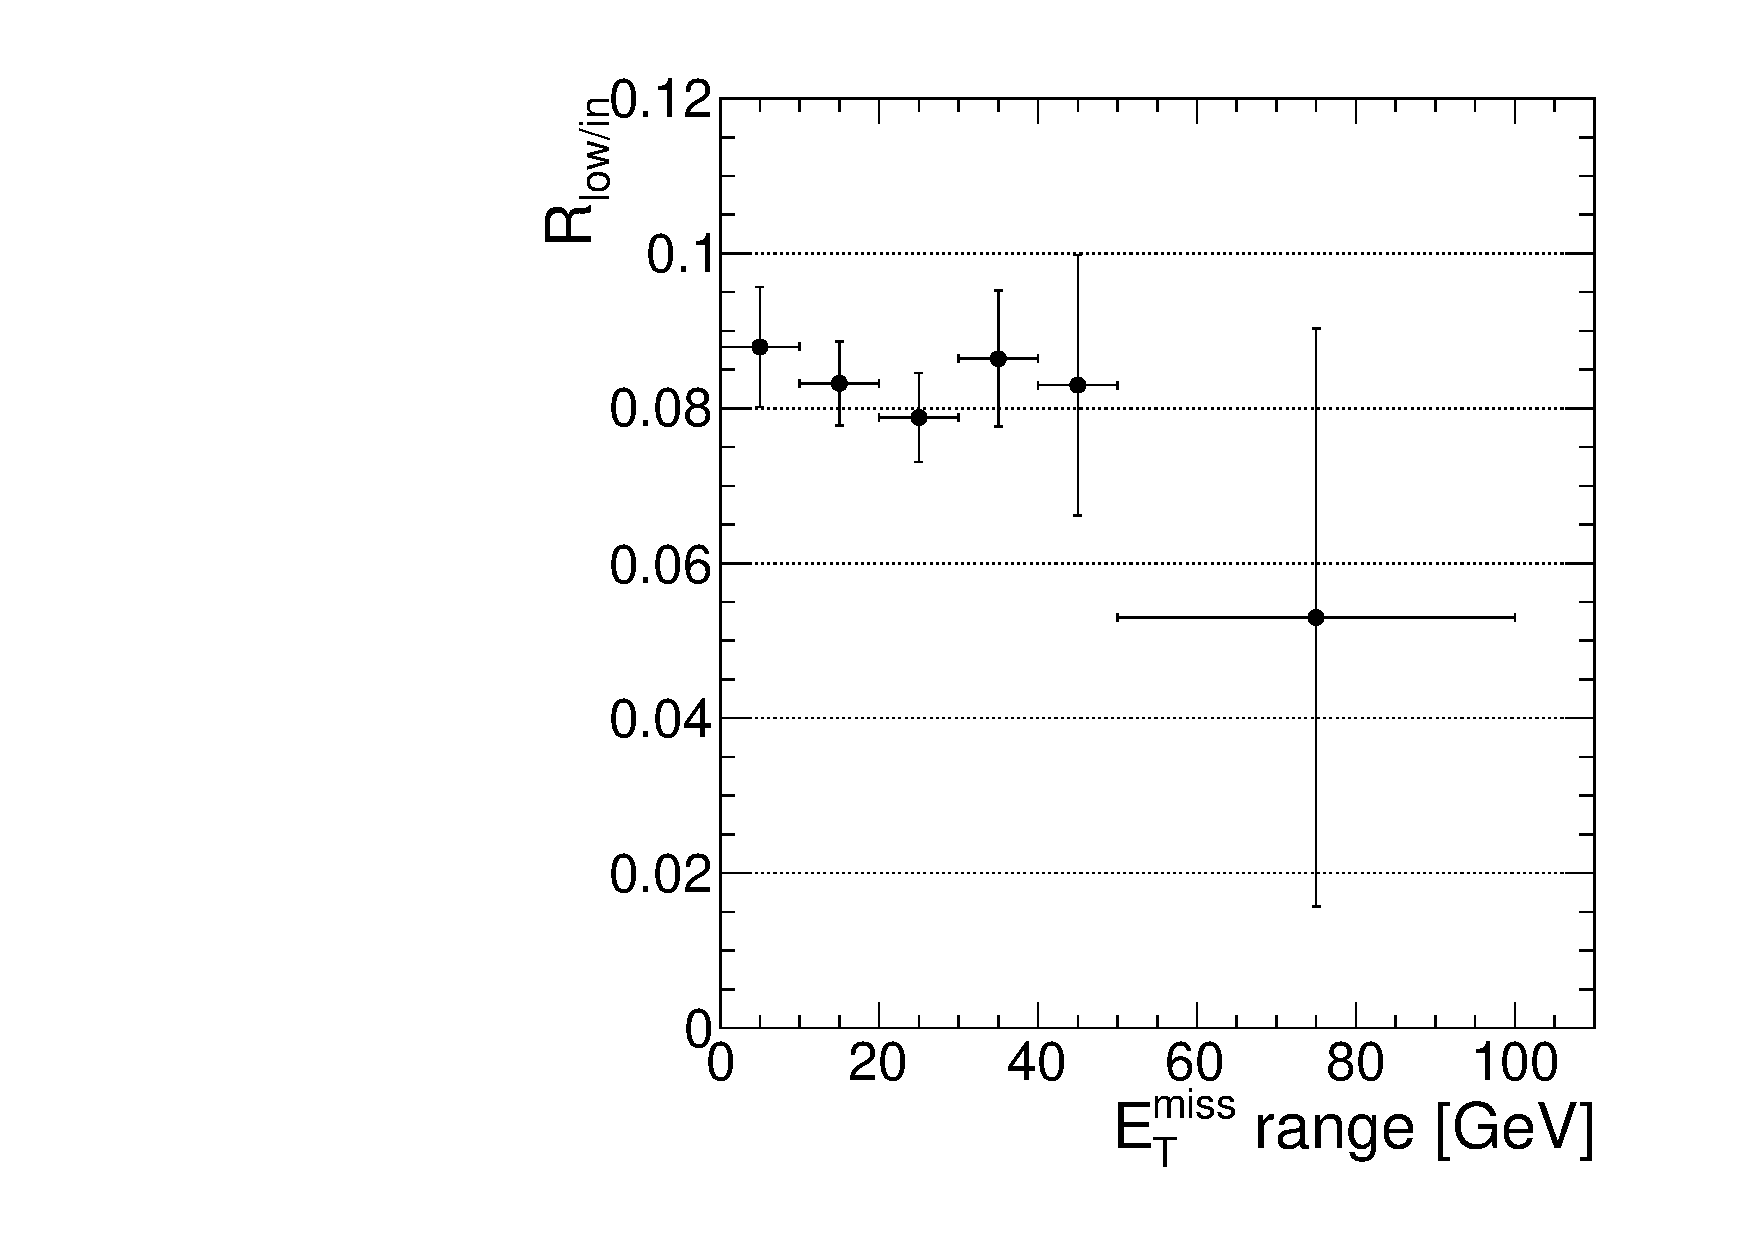
\includegraphics[width=0.4\textwidth]{plots/Routin_lowmet.pdf} &
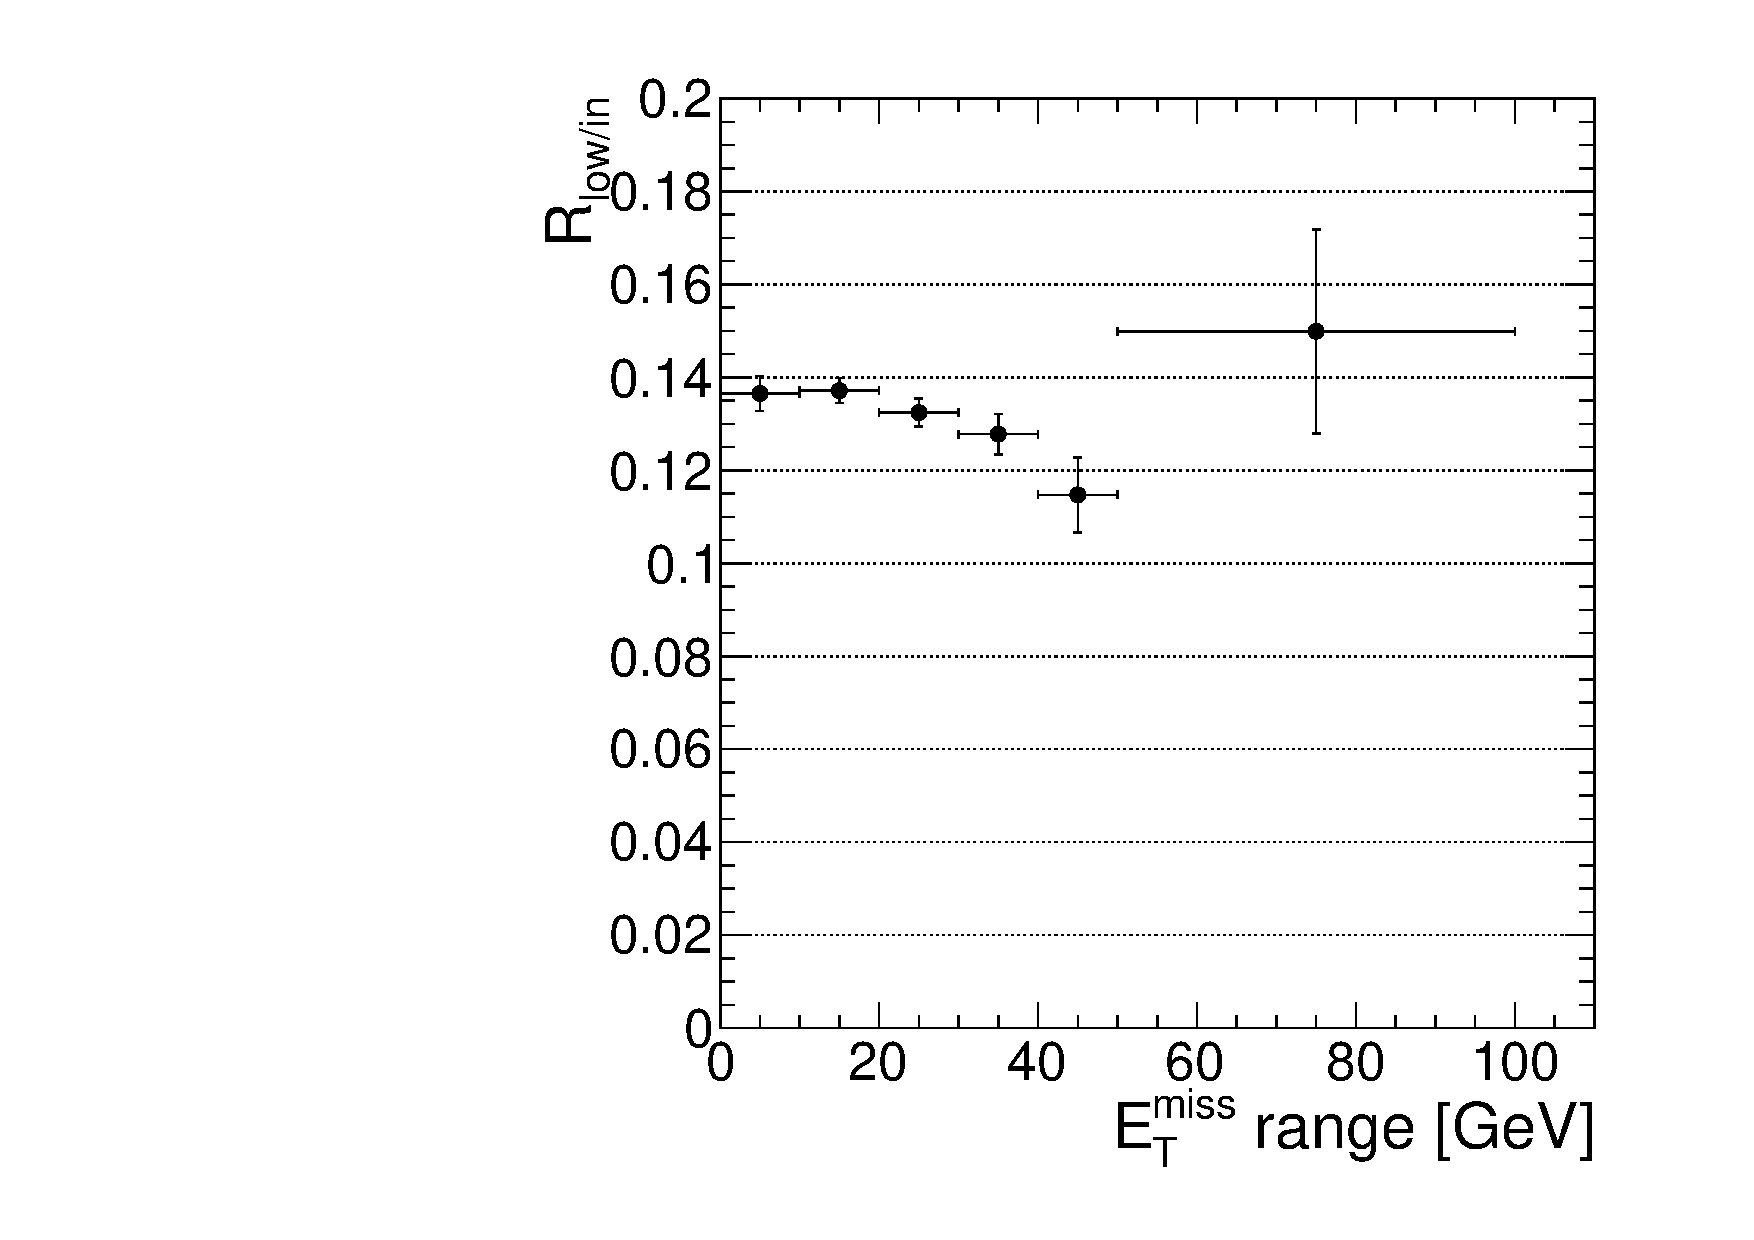
\includegraphics[width=0.4\textwidth]{plots/Routin_highMET.pdf} \\
\end{tabular}
\caption{\label{fig:Routin}
The ratio $R_{low/in}$ of low mass ($15<m_{\ell\ell}<70$ GeV) to on-Z ($81<m_{\ell\ell}<101$ GeV) events, as a function of
the \MET\ requirement. The left plot corresponds to the low \MET\ signal region (2 \pt\ $>$ 20 GeV leptons with at least 3 jets),
the right plot corresponds to the high \MET\ signal region (\pt\ $>$ (20,10) GeV leptons with at least 2 jets). 
}
\end{center}
\end{figure}

Given a prediction for the Z background in the Z mass window, we can extrapolate to estimate the low mass $\gamma^*$/Z contribution.
We extract the ratio $R_{low/in}$ of low-mass  to on-shell Z events from data,
correcting for the contribution from flavor-symmetric backgrounds, according to:

\begin{equation}
R_{low/in} = (N_{SF}^{low}-N_{OF}^{low})/(N_{SF}^{in}-N_{OF}^{in}).
\end{equation}

Here SF and OF refer to the same-flavor and opposite-flavor data yields in the ``low'' ($15<m_{\ell\ell}<70$ GeV) and ``in'' 
($81<m_{\ell\ell}<101$ GeV) dilepton mass regions. To predict the low-mass $\gamma^*$/Z contribution, we scale the total predicted
Z background by this quantity, which is displayed in Fig.~\ref{fig:Routin}. Here we measure $R_{low/in}$ in several \MET\ regions,
and assess the uncertainty based on the variation with respect to \MET. 
Based on this plot we choose $R_{low/in}=0.08\pm0.02$ for the low \MET\ signal region and $R_{low/in}=0.13\pm0.03$ for the high \MET\ region.

We find the following results for the first 5.1 fb$^{-1}$. For the low \MET\ signal region, the total predicted Z background in the Z mass region is $39\pm9.6$ 
(sum of the \zjets, WZ+ZZ, and rare SM backgrounds from Table~\ref{tab:results_lowmet}, \MET\ $>$ 100 GeV region), 
resulting in a $\gamma^*$/Z prediction of $3.1\pm1.1$ events. 
For the high \MET\ signal region, the total predicted Z background in the Z mass region is $30\pm8.1$ 
(sum of the \zjets, WZ+ZZ, and rare SM backgrounds from Table~\ref{tab:results_highmet}, \MET\ $>$ 150 GeV region), 
resulting in a $\gamma^*$/Z prediction of $3.8\pm1.4$ events. 

We find the following results for the full 9.2 fb$^{-1}$. For the low \MET\ signal region, the total predicted Z background in the Z mass region is $68\pm17$ 
(sum of the \zjets, WZ+ZZ, and rare SM backgrounds from Table~\ref{tab:results_edgefull}, \MET\ $>$ 100 GeV region), 
resulting in a $\gamma^*$/Z prediction of $5.4\pm1.9$ events. 
For the high \MET\ signal region, the total predicted Z background in the Z mass region is $60\pm16$ 
(sum of the \zjets, WZ+ZZ, and rare SM backgrounds from Table~\ref{tab:results_edgefull}, \MET\ $>$ 150 GeV region), 
resulting in a $\gamma^*$/Z prediction of $7.9\pm2.7$ events. 

\clearpage

\subsection{Summary of Results}
\label{sec:templates_summary}

In this section we summarize the results for the 5.1 fb$^{-1}$ Run2012A+B data (Table~\ref{tab:results_5p1})
and the 9.2 fb$^{-1}$ Run2012A+B+C data (Table~\ref{tab:results_9p2}).

\begin{table}[htb]
\begin{center}
\caption{\label{tab:results_5p1} Summary of results in 5.1 fb$^{-1}$ 2012A+B data for the low-\MET\ and high-\MET\ signal regions (SR).
In the Z mass region, the predicted Z background (Z bkg, sum of \zjets, WZ/ZZ, and rare SM processes with Z bosons), flavor-symmetric
background (FS bkg), and total background (Total bkg) are indicated, and compared to the observed yield (Data). 
The Gaussian significance of the difference between the data and the total background is indicated.
The predicted $\gamma^*/Z$ contribution to the low-mass region (Low mass $\gamma^*/Z$ bkg) is also indicated.}
\begin{tabular}{l|c|c}

\hline
\hline
& Low-\MET\ SR & High-\MET SR \\
\hline              
Z bkg                        & $39\pm9.6$          & $30\pm8.1$        \\
FS bkg                       & $99\pm16$           & $69\pm12$         \\
Total bkg                    & $138\pm18$          & $98\pm14$         \\
Data                         & 175                 & 95                \\
Significance                 & $+1.6\sigma$        & $-0.2\sigma$      \\
Low mass $\gamma^*/Z$ bkg    & $3.1\pm1.1$         &   $3.8\pm1.4$     \\
\hline
\hline

\end{tabular}
\end{center}
\end{table}

\begin{table}[htb]
\begin{center}
\caption{\label{tab:results_9p2} Summary of results in 9.2 fb$^{-1}$ 2012A+B+C data for the low-\MET\ and high-\MET\ signal regions (SR).
In the Z mass region, the predicted Z background (Z bkg, sum of \zjets, WZ/ZZ, and rare SM processes with Z bosons), flavor-symmetric
background (FS bkg), and total background (Total bkg) are indicated, and compared to the observed yield (Data). 
The Gaussian significance of the difference between the data and the total background is indicated.
The predicted $\gamma^*/Z$ contribution to the low-mass region (Low mass $\gamma^*/Z$ bkg) is also indicated.}
\begin{tabular}{l|c|c}

\hline
\hline
& Low-\MET\ SR & High-\MET SR \\
\hline              
Z bkg                        & $68\pm17$           & $60\pm16$         \\
FS bkg                       & $184\pm29$          & $117\pm20$        \\
Total bkg                    & $251\pm33$          & $177\pm25$        \\
Data                         & 288                 & 167               \\
Significance                 & $+1.0\sigma$        & $-0.4\sigma$      \\
Low mass $\gamma^*/Z$ bkg    & $5.4\pm1.9$         &   $7.9\pm2.7$     \\
\hline
\hline

\end{tabular}
\end{center}
\end{table}


\begin{comment}
The 5.1 fb$^{-1}$ results are summarized as:

\begin{itemize}
\item Low \MET\ signal region
\begin{itemize}
  \item Predicted Z background in Z mass region: $39\pm 9.6$ events
  \item Total predicted background in Z mass region: $138\pm18$ events
  \item Total observed yield in Z mass region: 175 events ($+1.6\sigma$)
  \item Low-mass $\gamma^*$/Z prediction: $3.1\pm1.1$ events
\end{itemize}
\item High \MET\ signal region
\begin{itemize}
  \item Predicted Z background in Z mass region: $30\pm 8.1$ events
  \item Total predicted background in Z mass region: $98\pm14$ events
  \item Total observed yield in Z mass region: 95 events ($-0.2\sigma$)
  \item Low-mass $\gamma^*$/Z prediction: $3.8\pm1.4$ events
\end{itemize}
\end{itemize}


The 9.2 fb$^{-1}$ results are summarized as:

\begin{itemize}
\item Low \MET\ signal region
\begin{itemize}
  \item Predicted Z background in Z mass region: $68\pm17$ events
  \item Total predicted background in Z mass region: $251\pm33$ events
  \item Total observed yield in Z mass region: 288 events ($+1.0\sigma$)
  \item Low-mass $\gamma^*$/Z prediction: $5.4\pm1.9$ events
\end{itemize}
\item High \MET\ signal region
\begin{itemize}
  \item Predicted Z background in Z mass region: $60\pm16$ events
  \item Total predicted background in Z mass region: $177\pm25$ events
  \item Total observed yield in Z mass region: 167 events ($-0.4\sigma$)
  \item Low-mass $\gamma^*$/Z prediction: $7.9\pm2.7$ events
\end{itemize}
\end{itemize}

\end{comment}

\clearpage


